\documentclass[a4paper,12pt]{article}
% Cabeçalho

% ABNT
\usepackage[utf8]{inputenc}
\usepackage[lmargin=3cm,tmargin=3cm,rmargin=2cm]{geometry}
\usepackage[singlespacing]{setspace}
\usepackage[T1]{fontenc}
\usepackage[brazil]{babel}
\usepackage{fancyhdr}
\usepackage{cite}
\usepackage{hyperref}

% Equações (necessário para as seções vindas do artigo do SIBGRAPI)
\usepackage{amsmath,amssymb}

% Pacotes esenciais
\usepackage{graphicx,subcaption,comment,enumerate,multirow,multicol,indentfirst}

% Comandos 


\bibliographystyle{plain}





\begin{document}

%Remove numeração da página atual
\thispagestyle{empty}

% Como fazer um cabeçalho passo a passo com tabular: https://www.youtube.com/watch?v=NEvF9mJwOXI&list=PLF6ZF9NW0WmqUAgtkYlQmCDHP6H_bYwGk&index=3

\begin{tabular}[l]{ll}
\multirow{5}*{
\includegraphics[width=50pt]{logo.png}} & 
\textbf{\resizebox{!}{0.3cm}{Universidade Federal do ABC}}\\&
\textbf{\resizebox{!}{0.25cm}{Av. dos Estados, 5001, Santa Terezinha, Santo André/SP, CEP 09210-580}}\\
\end{tabular}
\\
\\
\\
\\
\\
\\
\\
\\
\\
\\
\\
\\
\\
\\
\\
\\
\\

Relatório de Projeto de Graduação em Ciência da Computação
\\
\\
\\
\\
\\
\\
\textbf{Nome do aluno:} Felipe Nunes Carbone de Carvalho
\\
\\
\textbf{Nome do orientador:} João Paulo Gois
\\
\\
\textbf{Título do projeto:} Um novo pipeline unificado para Randomização de Domínio utilizando Gausian Splatting
\\
\\
\textbf{Palavras-chave do projeto:} \\ dataset sintético, gausian splatting, computação gráfica, inteligência artificial, aprendizado de máquina, randomização de domínio
\\
\textbf{Área do conhecimento do projeto:} \\ Computação Gráfica, Inteligência Artificial, Desenvolvimento de software

%Quebra de página
\newpage


%Sumário
\tableofcontents

\newpage

%Comando para determinar espaçamento entre linhas (1,5 nesse caso)
\onehalfspacing
{
%Define como tópico/seção do projeto (irá aparecer automaticamente no sumário)  
\section{Resumo}

A técnica de randomização de domínio (RD) para a criação de bases de dados sintéticos tem sido amplamente utilizada em contextos de visão computacional, principalmente em domínios onde a obtenção de dados reais se torna extremamente difícil ou mesmo inviável. Entretanto, ainda que esta técnica tenha se provado eficaz em diversas aplicações, o fato de ser focada na randomização das texturas dos objetos, que é o que garante a capacidade de generalização da silhueta destes, gera uma limitação evidente nos modelos de visão computacional treinados com este tipo de base de dados: A incapacidade de identificar padrões de textura e características anatômicas sutis devido à perda de informação ocasionada pela troca de textura do modelo, tais como padrões de venação alar em insetos ou padrões de cores que viabilizam a distinção entre espécies de animais, por exemplo. Visando resolver este problema, o presente trabalho apresenta uma nova técnica unificada para geração de dados sintéticos via RD que permite simultâneamente manter as vantagens da técnica tradicional que utiliza malhas 3D como modelos canônicos, bem como ampliar suas capacidades para a identificação de características para além da silhueta do objeto. Este resultado é obtido através da substituição das malhas por modelos gerados via Gausian Splatting. Ao realizar as randomizações de textura e iluminação diretamente nos parâmetros dos esféricos harmônicos associados às Gausianas 3D dos modelos, pode-se gerar tanto variações de textura similares às tradicionais, como também variações capazes de manter as estruturas complexas de padrões de cores e textura dos objetos originais. Dessa forma, datasets gerados com o pipeline proposto neste trabalho podem ser utilizados em uma variedade muito maior de domínios.

\section{Introdução}
Nos últimos anos, houve um grande avanço científico na aplicação de métodos de inteligência artificial, em particular no emprego de técnicas de aprendizado de máquina para a resolução de problemas em múltiplas áreas do conhecimento. As aplicações de métodos de aprendizado de máquina extrapolam as áreas de computação e engenharias e se estendem a áreas como medicina \cite{may2021eight}, biologia \cite{syen}, bioquímica \cite{mowbray2021machine}, física \cite{karniadakis2021physics}, sociologia \cite{di2021machine}, psicologia \cite{rosenbusch2021supervised}, entre outras. Esta característica multidisciplinar se deve principalmente a capacidade de generalização proporcionada pelos modelos de aprendizado de máquina.

Muitas aplicações de aprendizado de máquina utilizam modelos baseados em aprendizado supervisionado. Nessa metodologia, os modelos são construídos e treinados para uma aplicação específica a partir de exemplos. Cada exemplo consiste em uma amostra $x$ e um rótulo $y$ que a caracteriza. Esses exemplos formam um conjunto de dados, conhecido como \emph{dataset} \cite{Goodfellow-et-al-2016}.

A partir de exemplos conhecidos presentes no \emph{dataset}, o modelo é ajustado de maneira a aprender a distribuição estatística e as características inerentes aos dados. Um modelo treinado é capaz de generalizar o conhecimento sendo capaz de reconhecer e identificar o padrão de novos dados, que não foram vistos anteriormente no treinamento. 

Como os modelos que utilizam aprendizado supervisionado dependem de \emph{datasets} específicos a suas aplicações para extrair o conhecimento durante a fase de treinamento, estes dados são de extrema importância para o desenvolvimento destas aplicações. Um desafio recorrente a este tipo de abordagem é a disponibilidade de bases de dados anotados adequados à aplicação. Os dados devem possuir características que descrevam uma boa representação do problema, sendo necessário inevitavelmente uma grande quantidade deles.

A primeira dificuldade surge em obter dados em determinados domínios, pois muitas vezes não há dados públicos disponíveis e obter tais dados pode ser um trabalho árduo e até mesmo impraticável. Um exemplo prático para o contexto de visão computacional utilizando imagens pode ser dado para a área de medicina, no reconhecimento de características de uma doença rara, onde há poucas amostras disponíveis e obter novas amostras pode incorrer em altos custos, ou mesmo ser inesequível devido à baixa incidência da patologia. Mesmo quando há grande quantidade de amostras para uma determinada aplicação, outro problema recorrente é a atribuição de rótulos a essas amostras.

Valan et al. \cite{valan2021awakening} cita em seu trabalho o desafio de coletar amostras em quantidades suficientes de espécimes de insetos e a identificação de suas características, preservando a integridade das mesmas, devido à fragilidade destes animais, bem como seu tamanho, que pode chegar a poucos milímetros a depender da espécie, o que torna o processo custoso quanto a tempo e recursos humanos ou computacionais.

Para problemas onde as amostras são imagens, a atribuição de rótulos pode abranger desde identificação de objetos ilustrados na imagem em uma lista pré-determinada de objetos possíveis, até casos mais complexos de atribuir características que descrevam cada pixel da imagem. Nesses últimos casos, a atribuição de rótulos a uma única imagem pode demorar um tempo considerável, se tornando um problema para \emph{datasets} contendo milhares de exemplos.

A síntese de amostras e anotação utilizando técnicas de computação gráfica é uma forma de contornar a aquisição manual de amostras bem como sua anotação. A partir de um ambiente virtual 3D é possível criar imagens e vídeos sintéticos, onde há grande controle sobre o ambiente, pois nesses ambientes podemos controlar aspectos como posição da câmera e transformações de posição, escala e rotação de modelos 3D, além de rótulos por pixel de informações espaciais e semânticas, tais como profundidade, material, classe de objetos, entre outros. Tais características influenciam diretamente a qualidade e usabilidade dos dados no treinamento de redes neurais artificiais e outras técnicas de aprendizado de máquina.

Esta abordagem vem sendo utilizada por pesquisadores a fim de gerar grande quantidade de dados rotulados e se mostrou eficaz na generalização do aprendizado quando aplicados em métodos como redes neurais artificiais, redes de convolução, redes adversariais, entre outras \cite{Roberts_2021_ICCV, ros2016synthia, tremblay2018falling, Varol_2017_CVPR}. Estes trabalhos entretanto, realizam a síntese de cenas buscando a fidelidade com a realidade, o que gera a necessidade de um grande esforço humano na elaboração de modelos 3D e texturas, o que torna o processo demorado e custoso.

Para solucionar o problema de criação de datasets, surgiu a proposta da Randomização de Domínio. Essa abordagem utiliza distribuições aleatórias para gerar ambientes, texturas e transformações geométricas, com o objetivo de alcançar uma invariância de domínio nas imagens sintéticas geradas \cite{yue2019domain}. Essa extensa variação de parâmetros possibilita que modelos de inteligência artificial generalizem o problema, extraindo apenas as informações mais importantes das múltiplas variações possíveis \cite{Loquercio_2020}.

No caso de espécimes biológicos complexos, como insetos, a modelagem e a texturização 3D são particularmente difíceis. Esses objetos combinam estruturas unidimensionais (cerdas finas e antenas), estruturas planas bidimensionais (asas semitransparentes) e corpos volumétricos tridimensionais. Forçar essa geometria de dimensionalidade mista, juntamente com transparências complexas e texturas de alta frequência, em uma malha poligonal convencional frequentemente exige esforço manual e resulta em perda estrutural. Esse gargalo de representação é uma das principais razões pelas quais técnicas sem malhas, como o 3D Gaussian Splatting (3DGS), vêm ganhando espaço \cite{kerbl20233d}.

Além disso, em estudos de biodiversidade, a identificação automatizada de espécies sofre de um viés de textura, no qual os modelos de classificação dependem fortemente de padrões texturais locais em vez de estruturas morfológicas globais \cite{geirhos2018imagenettrained, bjerge2023accurate}. Superar esse viés é um desafio para os sistemas tradicionais de RD baseados em malhas \cite{tobin2017domain, blair2025leveraging}, uma vez que randomizar texturas para incentivar a generalização morfológica pode degradar pistas visuais essenciais à identificação taxonômica \cite{margapuri2021classification}.

A pesar do sucesso da RD, o fato de as randomizações de textura serem feitas sobre modelos de malhas 3D utilizando texturas aleatórias ou geradas a parir de ruido causam uma clara limitação na técnica: A perda das informação de textura do modelo randomizado. Ao randomizar as texturas dos objetos, as informações da textura original e muitas micro-estruturas do modelo se perdem, como por exemplo os padrões de venação alar em insetos, padrões específicos de coloração em animais e plantas, entre outros. Dessa forma, ainda que os modelos treinados com este tipo de dados tornem-se capazes de reconhecer as silhuetas das classes de treinamento eles não performam bem quando a distinção inter-classes depende destes padrões de coloração ou textura. Buscando atacar esta problemática, o presente trabalho apresenta uma nova técnica de RD baseada em modelos gerados via \emph{Gausian Splatting} aplicando perturbações nos modelos, mantendo características de cores e coerência de textura e transparência, o que viabiliza uma ampla randomização mantendo características essenciais para a classificação em domínios que exigem este tipo de informação.

Operando no espaço contínuo de parâmetros do 3DGS, o método proposto aplica dois \emph{pipelines} de perturbação independentes para sintetizar \emph{datasets} de treinamento randomizados. Primeiro, um \emph{pipeline} de RD Fotométrica aplica duas modulações distintas aos coeficientes de Harmônicos Esféricos (SH): altera o balanço de cores global deslocando as componentes de cor base e modifica a iluminação direcional incorporada, rotacionando a iluminação principal e escalando as reflexões especulares. Segundo, um \emph{pipeline} de RD Procedural isola a morfologia do objeto, substituindo suas texturas originais por ruído espacial 3D. Como a extração de \emph{bounding boxes} é essencial para o treinamento de arquiteturas de detecção \cite{deogan2025synthetic, ushiroji2026automatic}, elimina-se também a necessidade de anotação manual, extraindo as \emph{bounding boxes} 2D diretamente do motor de renderização.

Ao manipular o campo de radiância por meio desses \emph{pipelines}, o método gera \emph{datasets} sintéticos que preservam a integridade morfológica necessária para distinguir espécies biológicas, especialmente em grupos hiperdiversos e pouco conhecidos \cite{deep_darktaxa}. Essa abordagem pode padronizar o \emph{pipeline} de identificação biológica, permitindo um treinamento generalizado para descoberta de espécies e classificação taxonômica.

As principais contribuições deste trabalho são:
\begin{enumerate}
  \item Um \emph{pipeline} de RD sem malhas em dois estágios, que combina a manipulação \emph{offline} de parâmetros do 3DGS com rasterização independente em motor de jogos, automatizando a geração de \emph{datasets} anotados para identificação de espécies sem necessidade de extração de superfícies baseadas em malhas.
  \item Um \emph{pipeline} de RD Fotométrica que modula os SH por meio de matrizes D de Wigner de primeira ordem e escalonamento estocástico, para sintetizar variações de iluminação e de balanço de cores.
  \item Um \emph{pipeline} de RD Procedural que aplica ruído espacial 3D, preservando as primitivas geométricas subjacentes.
\end{enumerate}

\section{Fundamentação teórica}

\subsection{Randomização de Domínio} Á técnica de RD foi proposta pela primeira vez nos moldes atuais por \cite{tobin2017domain}, onde os pesquisadores adotaram pela primeira vez, não apenas uma variação randômica das posições dos objetos de estudo nas cenas, mas também uma randomização extensa de texturas e modelos sem compromisso com o foto realismo. Nesse trabalho, que tinha por objetivo tentar treinar um modelo para reconhecimento de objetos, visando o grande potencial de aplicação na operação de braços robóticos, mostrou-se que seria possível treinar modelos de redes neurais com bancos de dados sintéticos descompromissados com a realidade, desde que estes possuíssem suficiente variedade de cenários possíveis, apostando que se a quantidade de dados for grande e diversa o suficiente a rede neural treinada será capaz de identificar a realidade apenas como mais uma das variações possíveis mesmo sem nunca te-la observado. Os pesquisadores conseguiram resultados extremamente importantes sendo capazes de treinar o modelo com alta precisão. 

Uma vasta gama de trabalhos tem mostrado resultados promissores ao testar o desempenho da RD em comparação a outros tipos de \emph{datasets}. Um desses trabalho é \cite{tremblay2018training}, que buscou testar a eficácia de seu \emph{dataset} criado via RD contra duas outras bases de dados existentes. Nessa pesquisa o objetivo era treinar um modelo para reconhecimento de veículos no transito e como já existiam o \emph{KITTI dataset} \cite{doi:10.1177/0278364913491297} e o \emph{VKITTI dataset} \cite{gaidon2016virtual} para este fim, sendo o primeiro criado com imagens reais e o segundo com imagens geradas virtualmente com modelos 3D realistas, os pesquisadores puderam comparar o desempenho de seu modelo com essas duas formas alternativas de criação de bases de dados. O resultado, surpreendentemente, mostrou que o modelo treinado com RD foi capaz de superar em acurácia não apenas redes neurais treinadas com os \emph{datasets} \emph{KITTI}  ou o \emph{VKITTI}, mas também uma terceira rede treinada com abas simultaneamente, demonstrando que mesmo sendo uma opção menos custosa do que as outras duas opções, a RD possui potencial para igualar ou até mesmo superar os métodos alternativos. 

 Dado esse grande potencial demonstrado pela técnica de RD, diversos outros pesquisadores vem experimentando maneiras de utiliza-la para a geração de \emph{datasets} visuais, buscando encontrar quais parâmetros de randomização possuem maior influência no resultado final do treinamento das redes neurais \cite{valtchev2021domain, yue2019domain}, visando minimizar os custos de produção mantendo apenas as características mais relevantes para a eficácia do treinamento. Entre os parâmetros mais comumente utilizados estão as randomizações de textura, iluminação, posição e rotação de câmera, transformações de escala e uso de objetos distratores.

 Quanto aos parâmetros de randomização escolhidos comumente, não parece haver um padrão claro indicando seu impacto na eficiência do treinamento das redes neurais, com o desempenho podendo variar a depender da tarefa pretendida. Em \cite{james2017transferring}, por exemplo, a falta de objetos distratores no treinamento ocasionou na completa incapacidade do braço robótico realizar a tarefa de pegar um cubo e coloca-lo em uma cesta quando testado no mundo real, em contraste com acurácia próxima a 100\% observada ao utilizar objetos distratores na base de dadps de treinamento em conjunto aos outros parâmetros. Já em \cite{tremblay2018training} o uso de objetos distratores afetou a acurácia do modelo em identificar veículos em apenas 1\%.

 Há muito estabelecidos na robótica, esses \emph{frameworks} de dados sintéticos e randomização estão agora avançando para domínios biológicos \cite{margapuri2021classification, aghamohammadi2025blender}. Transpor esses \emph{pipelines} para cenários biológicos reais e complexos \cite{bjerge2023accurate}, no entanto, revela limitações críticas. \emph{Datasets} de biodiversidade existentes, como as coleções de mamíferos digitalizados em 3D \cite{blair2025leveraging}, podem depender de malhas explícitas no formato Wavefront associadas a texturas \emph{bitmap}. Essas representações são eficazes para estruturas macroscópicas difusas, mas falham em reproduzir com precisão as interações complexas entre luz e superfície da morfologia dos insetos, como reflexões especulares de alta frequência dependentes do ponto de vista, iridescência com variação espacial e a transmitância direcional de asas semitransparentes.
 

 \subsection{Gaussian Splatting}
 
 Introduzido por Kerbl et al.~\cite{kerbl20233d}, o 3D Gaussian Splatting (3DGS) representa cenas como coleções não estruturadas de gaussianas 3D anisotrópicas, capturando aparências dependentes do ponto de vista ao armazenar explicitamente coeficientes de Harmônicos Esféricos (SH). Embora essa representação reproduza bem as propriedades ópticas de objetos como carapaças biológicas, por exemplo, integrar o 3DGS em pipelines tradicionais de DR apresenta desafios estruturais. Converter campos de radiância baseados em pontos em malhas explícitas é um processo complexo. Métodos atuais de extração de superfície, como SuGaR~\cite{guedon2024sugar}, podem ter dificuldade em reconstruir sujeitos orgânicos detalhados, frequentemente comprometendo estruturas finas e semitransparentes (por exemplo, asas de insetos e cerdas) e perdendo as propriedades de iluminação incorporadas nos primitivos.

Embora revisões recentes destaquem a rápida adoção do 3DGS em domínios como segmentação, modelagem generativa e robótica \cite{he2026survey, chen2026survey}, sua aplicação como motor nativo e procedural de síntese de dados permanece amplamente inexplorada. Esforços recentes \cite{deogan2025synthetic, ushiroji2026automatic} começaram a utilizar modelos 3DGS como \emph{assets} estáticos em motores de jogos; entretanto, essa abordagem não explora plenamente o potencial da parametrização de campos de radiância. Por outro lado, a extração de superfícies, estratégia comum para conectar o 3DGS aos \emph{pipelines} de RD baseados em malhas, degrada inerentemente estruturas biológicas semitransparentes e incorpora de forma permanente a iluminação dependente do ponto de vista em texturas estáticas. Essa perda na conversão geométrica evidencia a necessidade de \emph{frameworks} de RD que operem diretamente sobre representações de radiância baseadas em pontos, evitando por completo o gargalo da extração de malhas. A parametrização explícita do 3DGS, aliás, já foi identificada como um espaço de trabalho controlável para a manipulação de cenas, sendo utilizada, por exemplo, para calcular propriedades de materiais e da cena \cite{liang2024gsir, Gao2025Relightable}.

Embora modelos 3DGS treinados sejam inerentemente estáticos, trabalhos recentes utilizaram matrizes de Wigner D para manter a consistência de iluminação durante a animação de avatares humanos articulados \cite{hu2024gauhuman, gkitsas2024skinning}. Neste trabalho, adaptamos essa propriedade matemática como um mecanismo estocástico de re-iluminação para geração de dados sintéticos em geometria estática.

Tendo em vista o carater estático inerente aos modelos 3DGS, a literatura recente tem explorado a perturbação direta de seus parâmetros subjacentes. No contexto de robustez adversarial e marca d'água digital, métodos como \textit{3DGAA} \cite{wang20243dgaa}, \textit{MPAM-3DGS} \cite{jiang2024mpam} e \textit{GaussianMarker} \cite{huang2024gaussianmarker} alteram propriedades espaciais e de cor para avaliar a robustez da rede ou embutir dados ocultos. Para a reconstrução de cenas dinâmicas, métodos como \textit{GauHuman} \cite{hu2024gauhuman} e \textit{Skinned Gaussian Avatars} \cite{gkitsas2024skinning} aplicam matrizes D de Wigner para compensar a rotação de geometrias articuladas, mantendo a consistência da iluminação. Baseando-se nessas operações em espaço de parâmetros, nosso \textit{framework} adapta perturbações matemáticas explícitas especificamente para a síntese de dados, funcionando como um mecanismo para a randomização de domínio fotométrico e geométrico.

Funções de ruído procedural, como o ruído de Perlin e Simplex \cite{perlin1985image}, são amplamente utilizadas em computação gráfica para a geração de texturas orgânicas, sendo tipicamente avaliadas sobre coordenadas UV bidimensionais. Em renderização neural e representações volumétricas, o ruído estrutural tem sido empregado para simular meios participantes e espalhamento atmosférico. Nosso \textit{framework} aplica este conceito a campos de radiância explícitos, avaliando o ruído espacial 3D diretamente sobre as coordenadas espaciais não estruturadas das Gaussianas. Isso trata o campo de radiância como um espaço volumétrico para variação morfológica procedural e degradação óptica, permitindo a randomização de domínio estrutural sem depender de parametrização de superfície.

 

\section{Metodologia}
Dado o objetivo deste trabalho de gerar e validar bases de imagens sintéticas para o domínio de identificação e classificação de espécies de insetos a partir de modelos de 3D Gaussian Splatting, propôs-se uma estrutura metodológica dividida em seis partes, e baseada em duas ferramentas distintas, sendo elas:

\subsection{Geração de modelos 3DGS canonicos}
Para obter os modelos 3DGS canonicos, isto é, os modelos base sobre os quais a 
randomização de domínio atuará nas proximas etapas, foram capturadas sequências 
de imagens dos espécimes biológicos utilizando dispositivos
móveis convencionais (um Motorola Edge 30 Fusion para o espécime de mosca e um
Samsung Galaxy S24 para a mariposa). Em ambos os casos as imagens foram retiradas 
a partir de vídeos gravados ao rotacionar a camera ao redor do animal.

Estes modelos canônicos foram reconstruídos
a partir das implementações prontas do SuGaR~\cite{guedon2024} (dispensando a etapa
opcional de extração de malha, de modo a manter a representação puramente em
\textit{splats}) e do EFA-GS~\cite{wang2025}. Como nossa contribuição central
reside na randomização de domínio de campos de radiância, e não na fase de
reconstrução em si, utilizamos os parâmetros de otimização padrão fornecidos por
esses \textit{frameworks}. Os modelos 3DGS brutos foram então importados no
editor SuperSplat~\cite{supersplat}, onde foi realizado uma poda
manual para isolar a morfologia dos espécimes, removendo a geometria do fundo e
\textit{floaters} periféricos (Fig.~\ref{fig:base}).

\begin{figure}[htb]
  \centering
  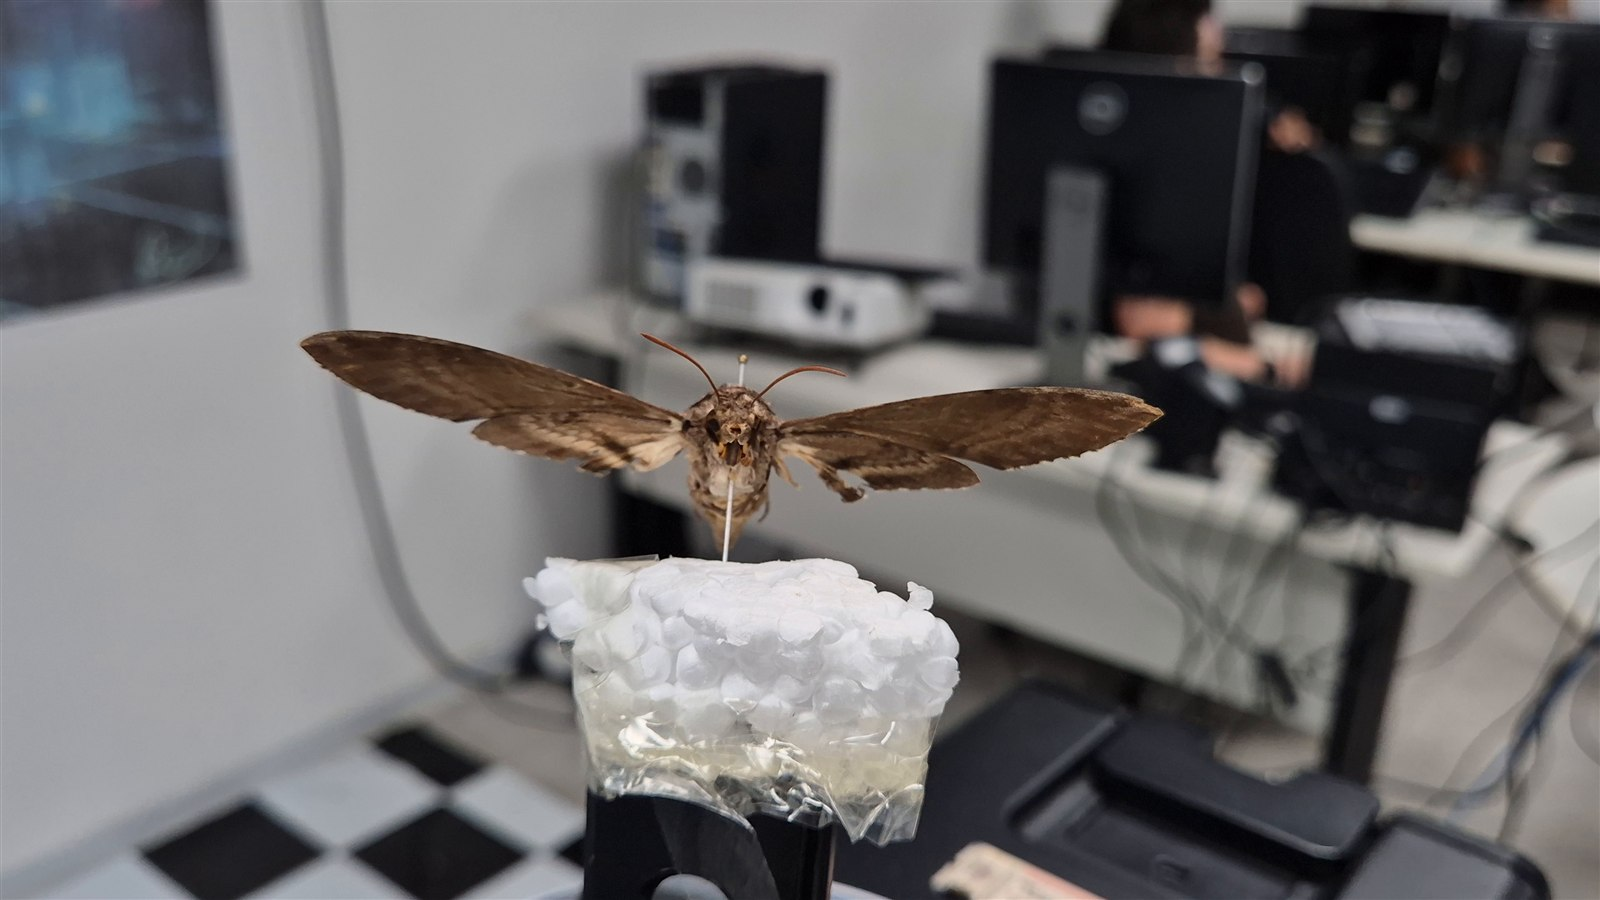
\includegraphics[width=0.49\linewidth]{imagens/artigo/im1.jpg}\hfill
  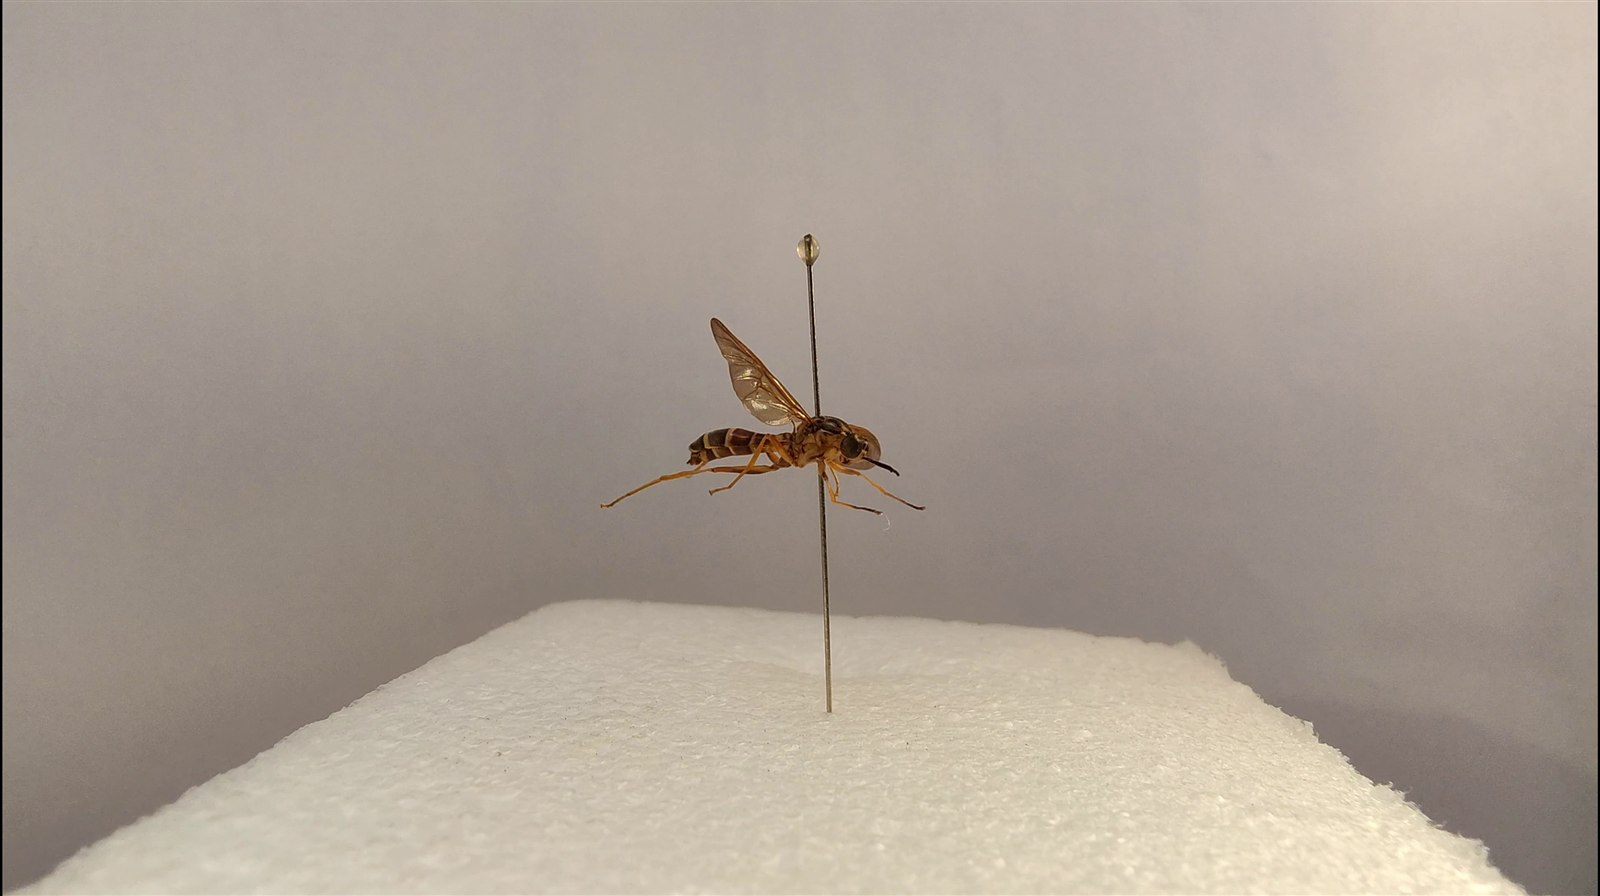
\includegraphics[width=0.49\linewidth]{imagens/artigo/im2.jpg}\\[2pt]
  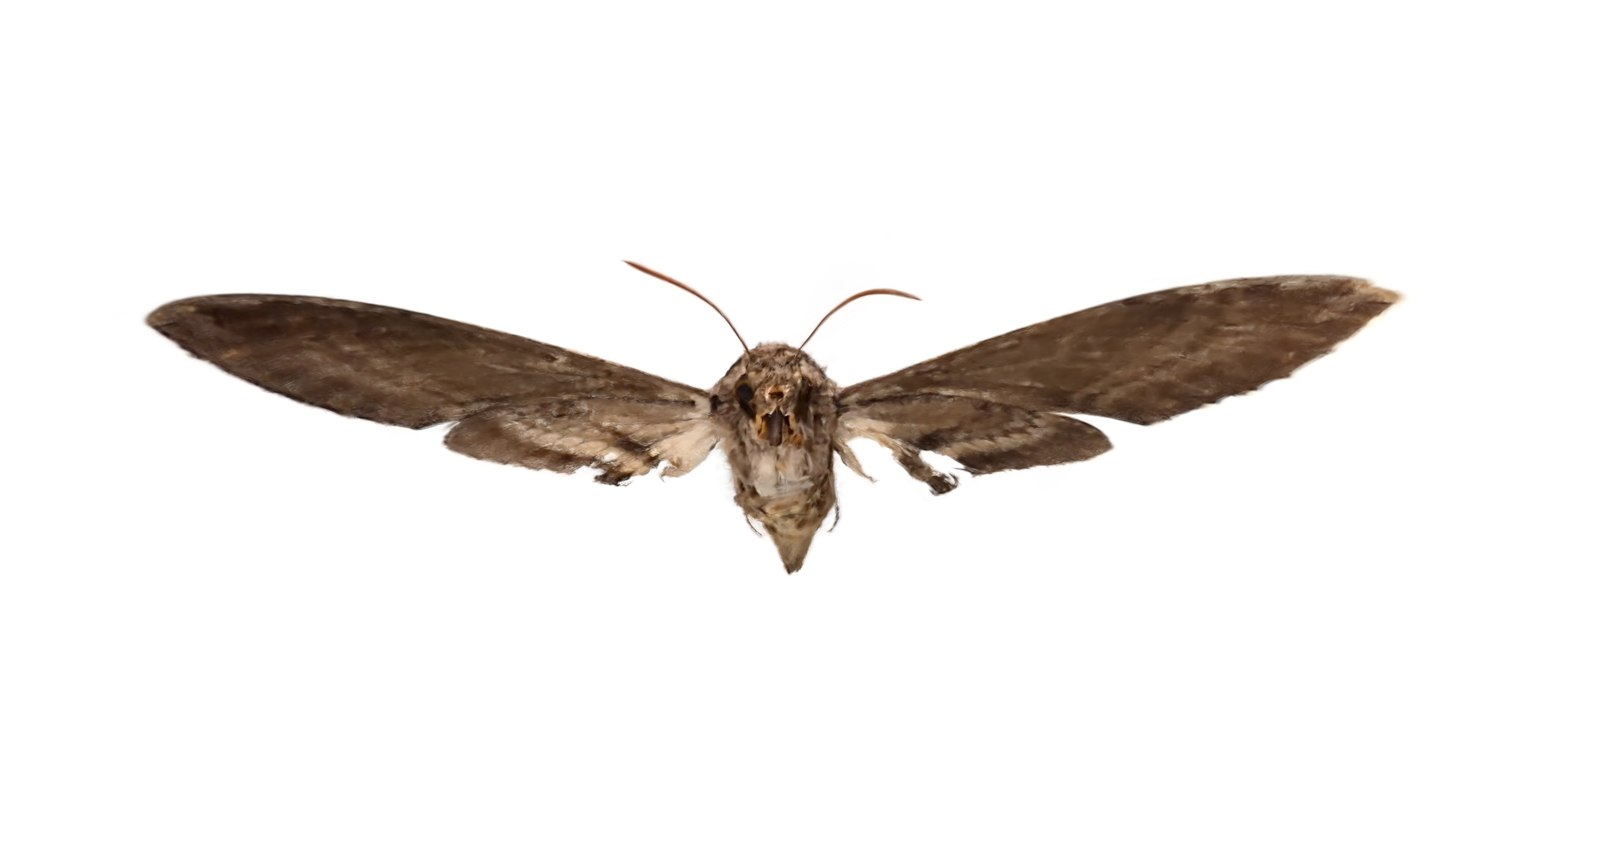
\includegraphics[width=0.49\linewidth]{imagens/artigo/im3.jpg}\hfill
  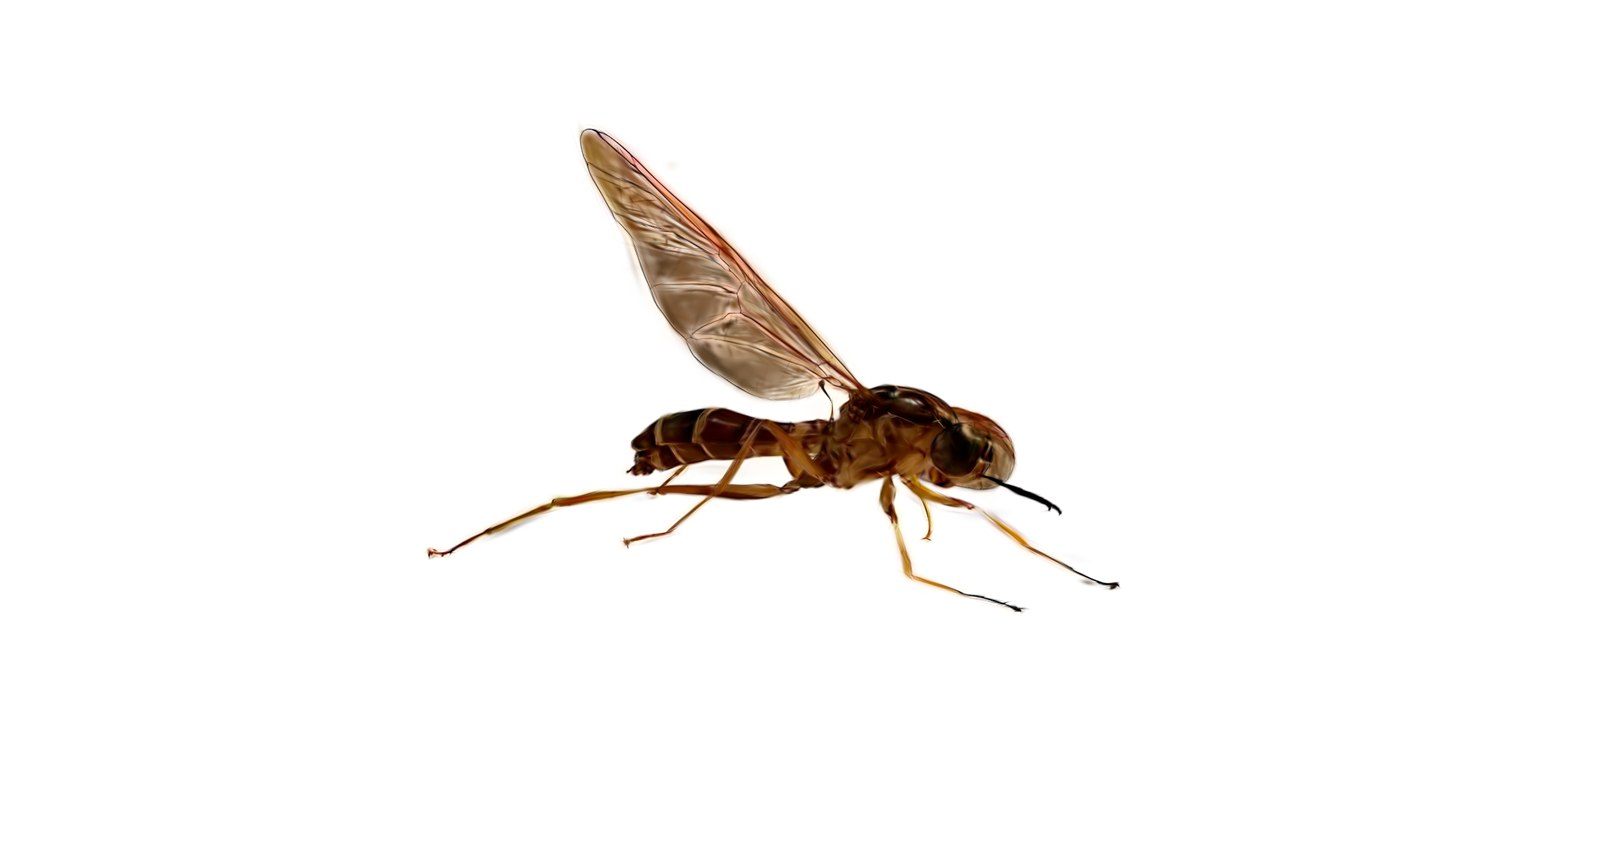
\includegraphics[width=0.49\linewidth]{imagens/artigo/im4.jpg}
  \caption{Reconstruções 3DGS de base. Acima: \emph{frames} representativos de vídeos multivista capturados à mão livre de uma mariposa e de uma mosca com dispositivos móveis. Abaixo: os modelos canônicos de 3D Gaussian Splatting correspondentes, recortados manualmente para isolar as estruturas morfológicas antes da perturbação dos parâmetros.}
  \label{fig:base}
\end{figure}

Antes da aplicação das perturbações estocásticas, executa-se uma etapa de poda espaço-óptica para refinar o modelo base, inspirada em técnicas de filtragem estrutural utilizadas para mitigar \textit{floaters} e artefatos de renderização \cite{kerbl20233d, hu2024gauhuman, wang20243dgaa}. Embora \textit{splats} de baixa opacidade e muito alongados sejam frequentemente imperceptíveis na reconstrução original, eles representam um risco durante a randomização de domínio: quando operações estocásticas, como deslocamentos agressivos de cor ou substituição por ruído procedural, são aplicadas, esses artefatos latentes podem ser amplificados, criando ruído visual que degrada a silhueta e os detalhes estruturais do objeto. Para evitar essa deterioração, removem-se os \textit{splats} que apresentam simultaneamente opacidade inferior a 10\% e alongamento espacial extremo, definido como o maior eixo principal excedendo 10 vezes o menor. Esses limiares são hiperparâmetros empíricos que podem ser ajustados para cada conjunto de dados. Além disso, essa etapa é opcional e pode ser dispensada caso os modelos 3DGS estejam livres de artefatos.

Após o isolamento manual dos modelos 3DGS brutos gerados a partir do SuGaR, aplicamos nossa etapa de poda (etapa opcional que pode ou não ser habilitada de acordo com a necessidade), o resultado desta etapa é o que chamamos modelo canônico.

Inicialmente, o modelo da mariposa era composto
por 154.330 \textit{splats} e o da mosca, por 15.413 \textit{splats}. Após a
remoção dos artefatos de baixa opacidade e muito alongados, os modelos foram
reduzidos a 95.406 e 9.166 \textit{splats}, respectivamente, resultando em
\textit{priors} geométricos mais limpos, poupando processamento e mantendo a estrutura original dos modelos.




\subsection{Geração dos modelos DR com colab}

Os modelos randomizados são gerados aplicando perturbações diretamente ao espaço de parâmetros dos modelos 3DGS canônicos. Os tensores de parâmetros perturbados estocasticamente são pré-calculados em Python e exportados como arquivos \texttt{.ply} individuais, que são posteriormente carregados no motor Unity para a geração dos \emph{datasets}.

Considere um modelo 3DGS com $N$ primitivas gaussianas individuais, com atributos geométricos e volumétricos: posição $\boldsymbol{\mu} \in \mathbb{R}^{N\times 3}$, escala anisotrópica $\mathbf{s} \in \mathbb{R}^{N\times 3}$, quatérnios de rotação $\mathbf{q} \in \mathbb{R}^{N\times 4}$ e opacidade $\boldsymbol{\alpha} \in \mathbb{R}^{N}$. Seguindo Kerbl et al.~\cite{kerbl20233d}, as propriedades ópticas dependentes do ponto de vista são modeladas por coeficientes de Harmônicos Esféricos (SH) $\mathbf{c} \in \mathbb{R}^{N\times 16\times 3}$.

Para executar perturbações diretamente nesse espaço multidimensional, os parâmetros SH são categorizados de acordo com seu grau $\ell$. O grau $\ell = 0$ representa a cor base independente do ponto de vista (análoga ao albedo intrínseco), enquanto graus superiores ($\ell > 0$) capturam reflexões direcionais de alta frequência dependentes do ponto de vista. A partir dessa categorização, são aplicados dois \emph{pipelines} de perturbação independentes, descritos a seguir.

\subsubsection{Pipeline A: RD Fotométrica}

São calculados dois operadores sobre os SH que desacoplam o balanço de cor difusa das reflexões especulares dependentes do ponto de vista.

\paragraph{Deslocamento fotométrico de cor.} Inspirado em modelos de modificação fotométrica e corrupção utilizados em robustez adversarial \cite{wang20243dgaa}, simulam-se balanços de cor de sensores e variações de iluminação aplicando um fator de escala global $\gamma$ e um deslocamento de cor $\boldsymbol{\delta}_{\text{cor}}$ à componente DC ($\ell = 0$):
\begin{equation}
  \hat{\mathbf{c}}_{00} = \gamma\,\mathbf{c}_{00} + \boldsymbol{\delta}_{\text{cor}},
\end{equation}
em que $\mathbf{c}_{00} \in \mathbb{R}^{3}$ representa os coeficientes DC originais da primitiva gaussiana e $\gamma \in \mathbb{R}$ é um fator escalar estocástico que simula variações globais de exposição. O vetor de perturbação é amostrado de uma distribuição uniforme sobre o espaço SH irrestrito, de modo que $\boldsymbol{\delta}_{\text{cor}} \in [-1{,}2;\, 1{,}2]^{3}$. Esse intervalo é um hiperparâmetro empírico ajustado para espécimes biológicos; como esses deslocamentos são aplicados diretamente aos parâmetros brutos, antes das etapas de projeção e saturação (\emph{clamping}) do rasterizador, eles permitem uma simulação de alta variância de deslocamentos extremos de balanço de branco, preservando os gradientes estruturais locais contra a saturação prematura dos \emph{pixels}.

\paragraph{Rotação de Wigner das componentes AC e escalonamento especular.} Para simular a rotação das fontes de luz principais, adaptam-se conceitos de rotação de SH explorados em avatares articulados \cite{hu2024gauhuman, gkitsas2024skinning} para geometrias estáticas. Embora rotacionar todas as bandas SH por meio de matrizes D de Wigner seja matematicamente rigoroso \cite{gkitsas2024skinning}, aplicar essas transformações aos coeficientes de ordem superior gera benefícios visuais decrescentes diante de seu alto custo computacional \cite{hu2024gauhuman}. Assim, para manter um equilíbrio entre qualidade visual e vazão de renderização na síntese de dados, a rotação explícita da iluminação é restrita à iluminação direcional principal (grau $\ell = 1$), para a qual a matriz D de Wigner se reduz a uma rotação cartesiana $3\times 3$ padrão, $\mathbf{R}$ \cite{gkitsas2024skinning}. As componentes AC de ordem superior ($\ell > 1$) não passam por essa rotação e são moduladas apenas por um fator estocástico de escala especular log-normal, $\sigma_{\text{spec}}$. Os coeficientes AC atualizados são calculados como:
\begin{equation}
  \hat{\mathbf{c}}_{\ell} =
  \begin{cases}
    \sigma_{\text{spec}}\,\mathbf{R}\,\mathbf{c}_{\ell}, & \ell = 1,\\[2pt]
    \sigma_{\text{spec}}\,\mathbf{c}_{\ell}, & \ell > 1.
  \end{cases}
\end{equation}

\subsubsection{Pipeline B: RD Procedural}

Para obter randomização estrutural e garantir que nenhuma pista textural dependente do ponto de vista se propague para a representação procedural, a componente de cor DC é substituída e todas as componentes AC de ordem superior são zeradas:
\begin{equation}
  \hat{\mathbf{c}}_{\ell} =
  \begin{cases}
    \tau\!\left(\mathcal{N}(\boldsymbol{\mu}_i)\right)\cdot \mathbf{C}_{\text{amp}} + \mathbf{C}_{\text{shift}}, & \ell = 0,\\[2pt]
    \mathbf{0}, & \ell > 0,
  \end{cases}
\end{equation}
em que $\mathcal{N}(\boldsymbol{\mu}_i)$ representa uma função de ruído espacial 3D multiescala avaliada na posição média $\boldsymbol{\mu}_i$ da $i$-ésima gaussiana. Para incentivar uma ampla gama de padrões texturais, a função de transformação $\tau(\cdot)$ aplica estocasticamente ou uma função degrau com limiar randomizado, binarizando o ruído em manchas estruturais discretas, ou um mapeamento identidade, que preserva gradientes contínuos de cor. Por fim, os parâmetros escalados dinamicamente $\mathbf{C}_{\text{amp}}$ e $\mathbf{C}_{\text{shift}}$ mapeiam linearmente os padrões resultantes em espaços de cor randomizados.

As Figuras~\ref{fig:fotometrica} e~\ref{fig:procedural} apresentam exemplos das saídas de cada \emph{pipeline}.

\begin{figure}[htb]
  \centering
  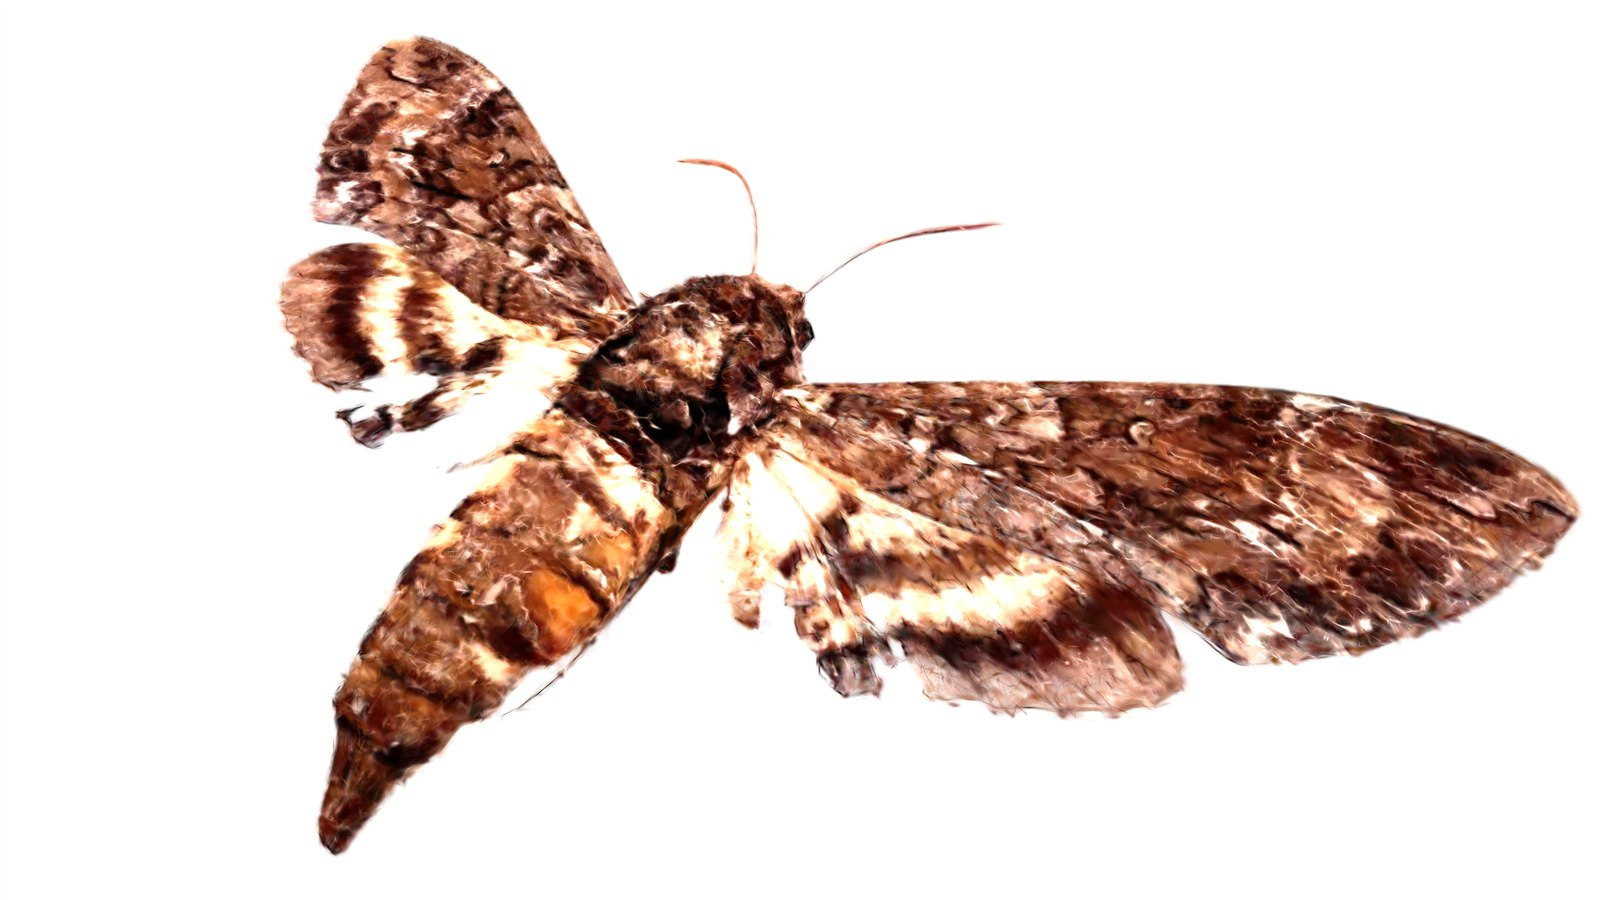
\includegraphics[width=0.24\linewidth]{imagens/artigo/im5.jpg}\hfill
  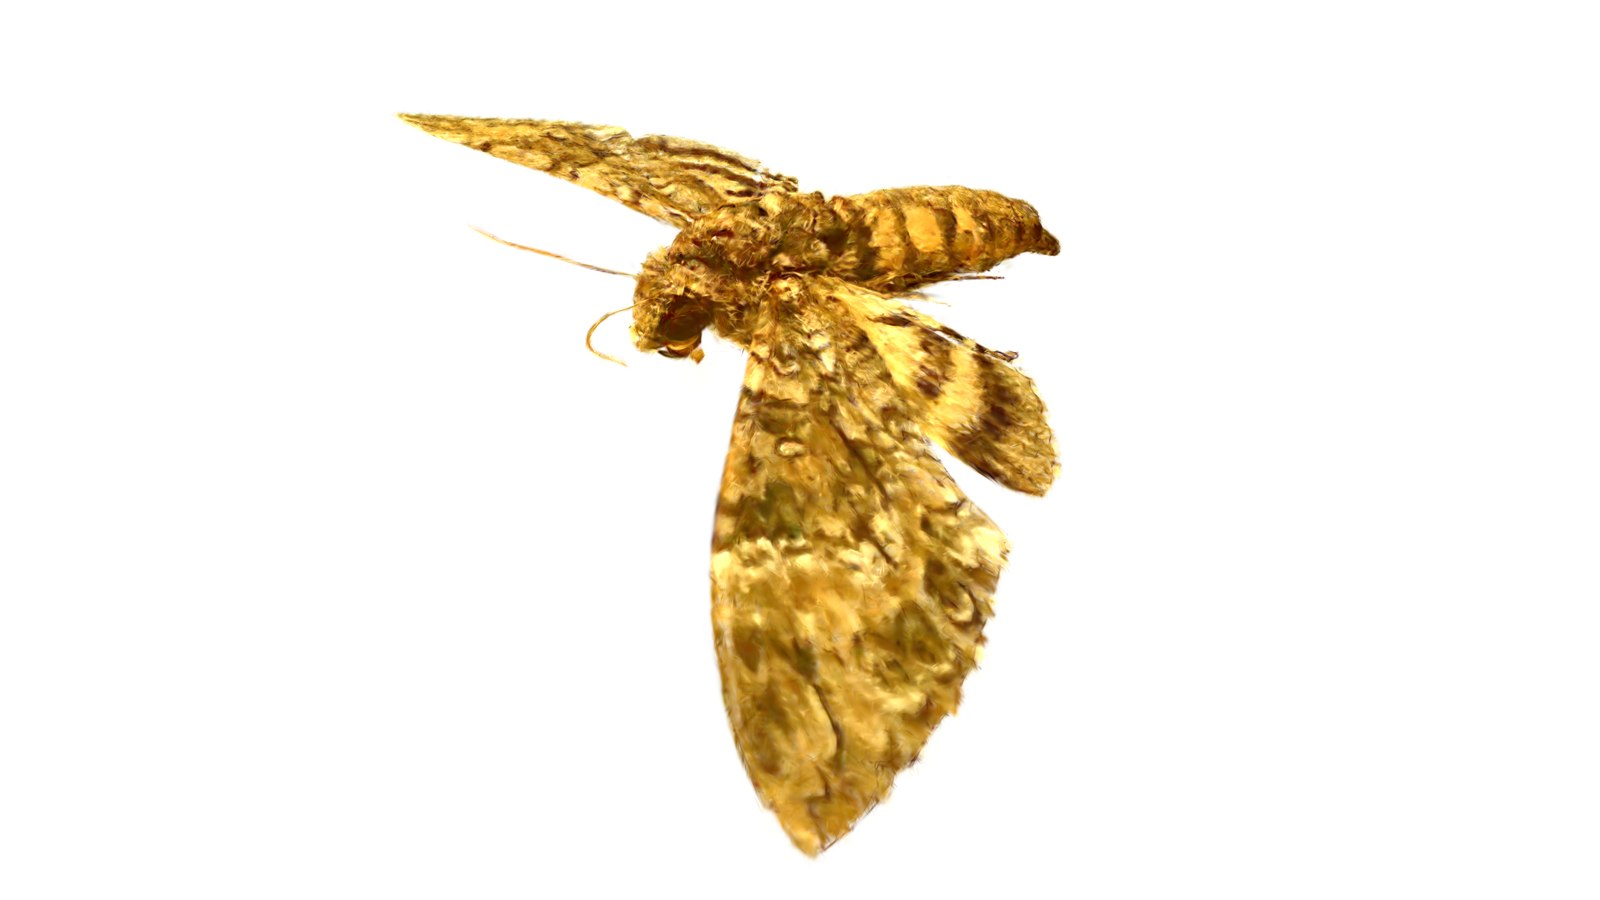
\includegraphics[width=0.24\linewidth]{imagens/artigo/im6.jpg}\hfill
  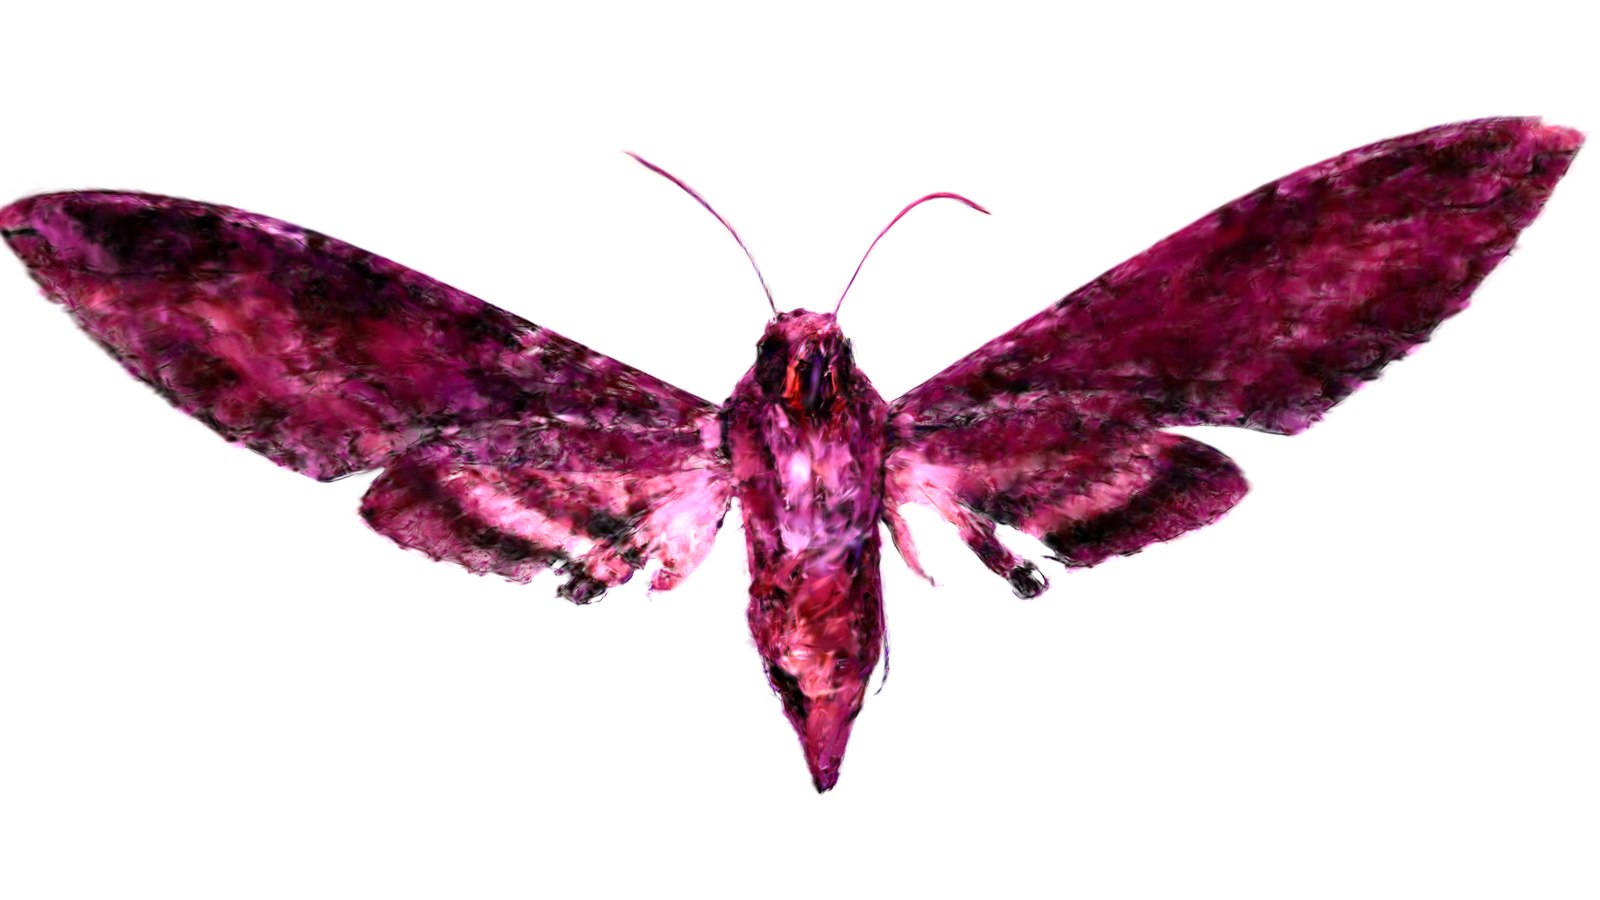
\includegraphics[width=0.24\linewidth]{imagens/artigo/im7.jpg}\hfill
  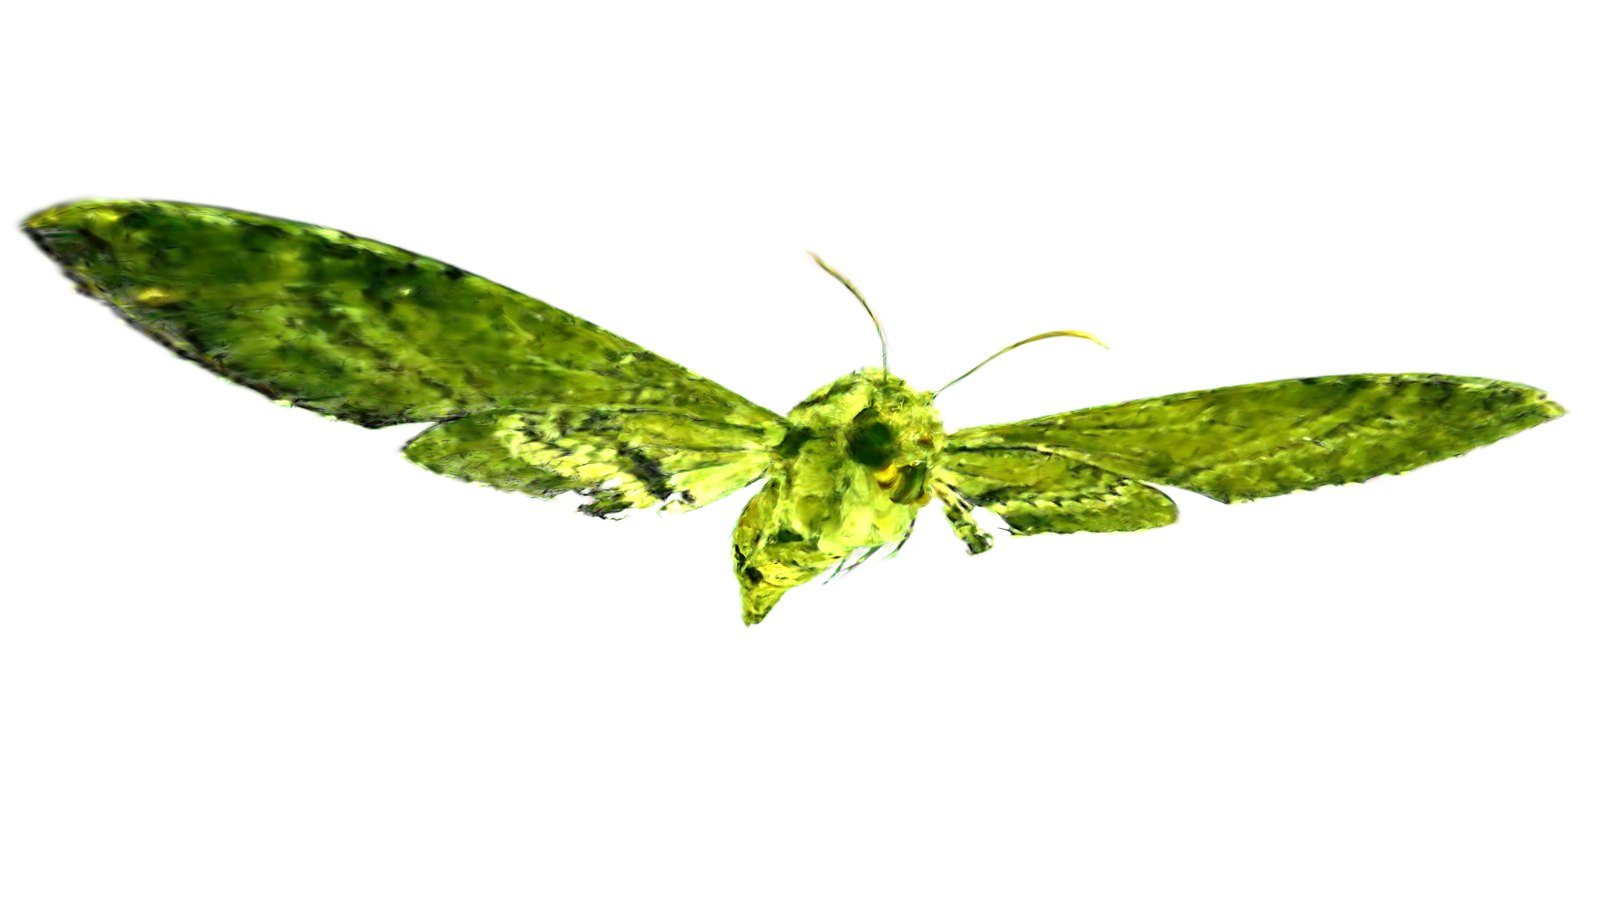
\includegraphics[width=0.24\linewidth]{imagens/artigo/im8.jpg}\\[2pt]
  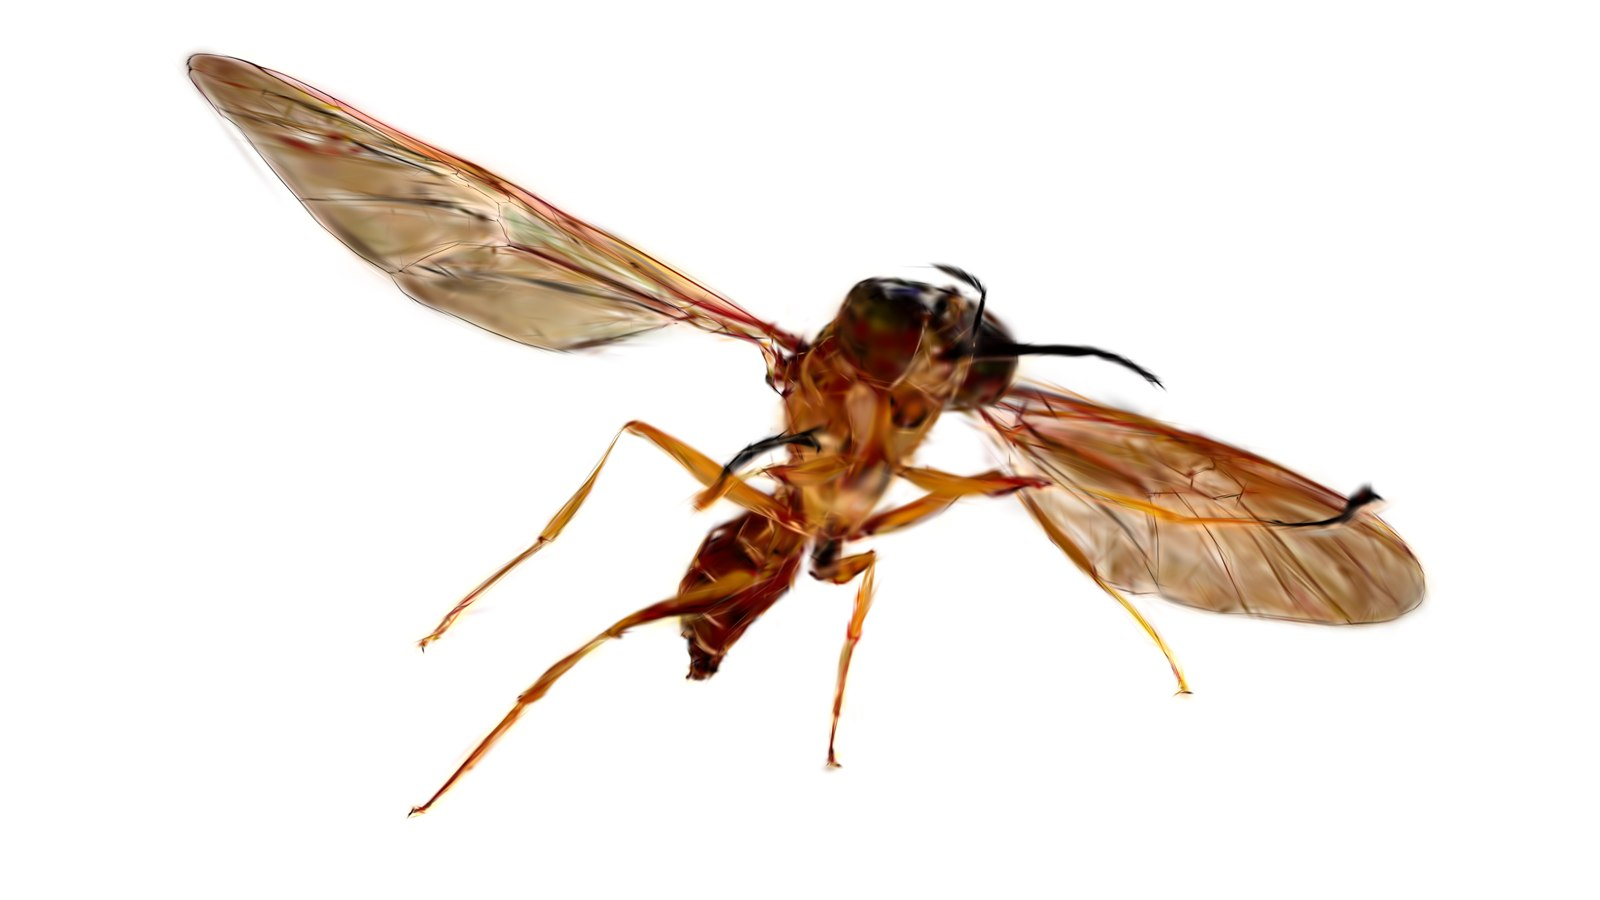
\includegraphics[width=0.24\linewidth]{imagens/artigo/im9.jpg}\hfill
  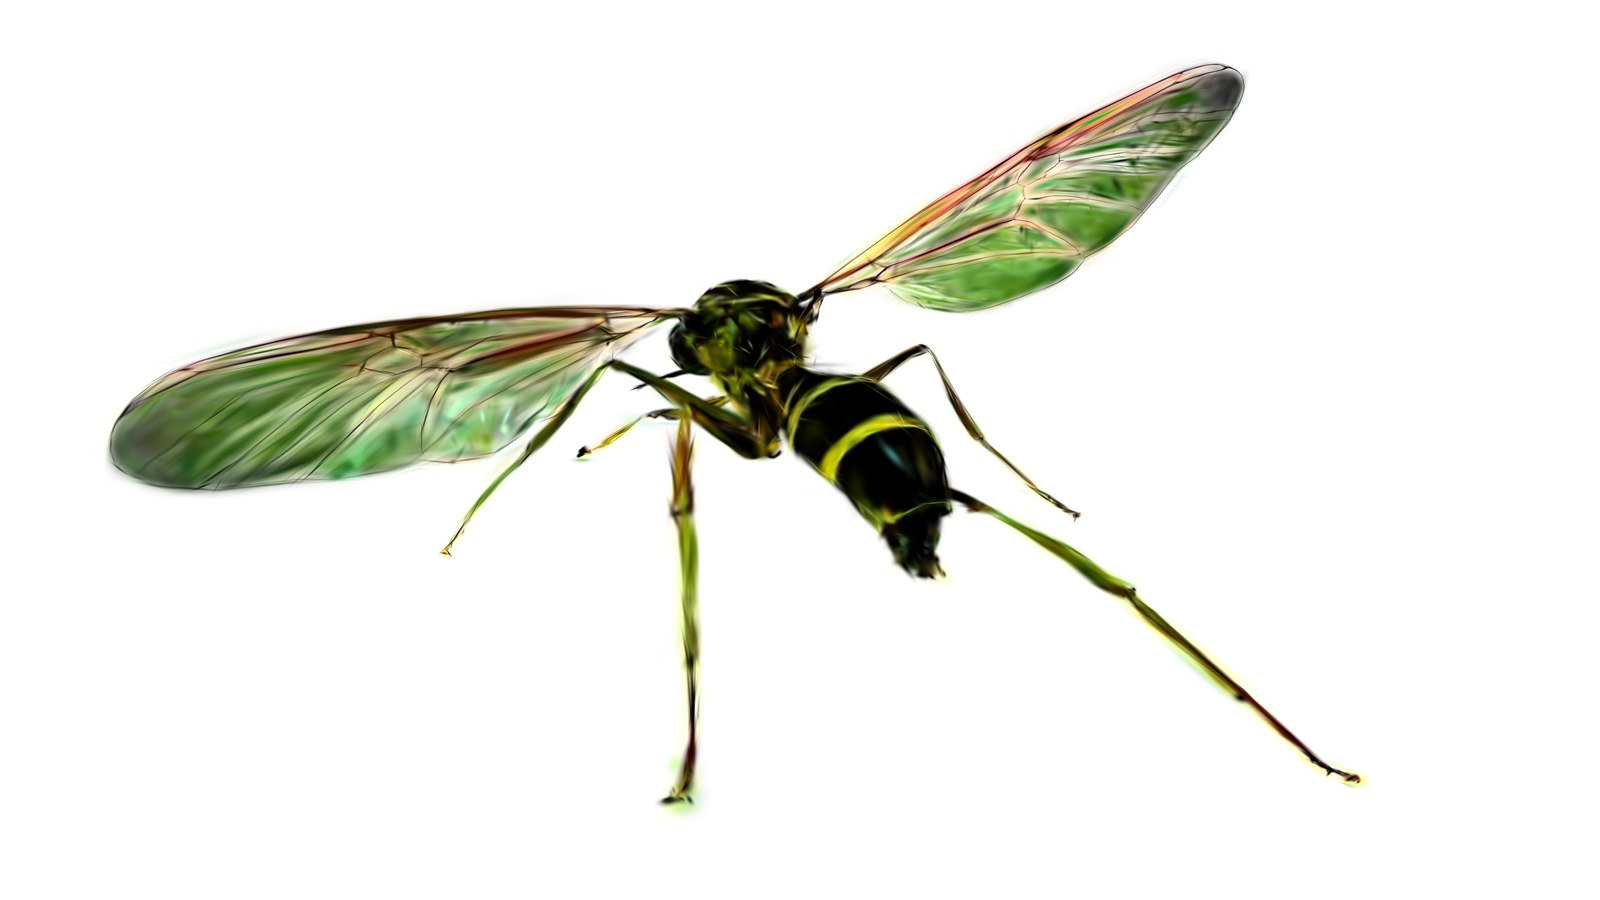
\includegraphics[width=0.24\linewidth]{imagens/artigo/im10.jpg}\hfill
  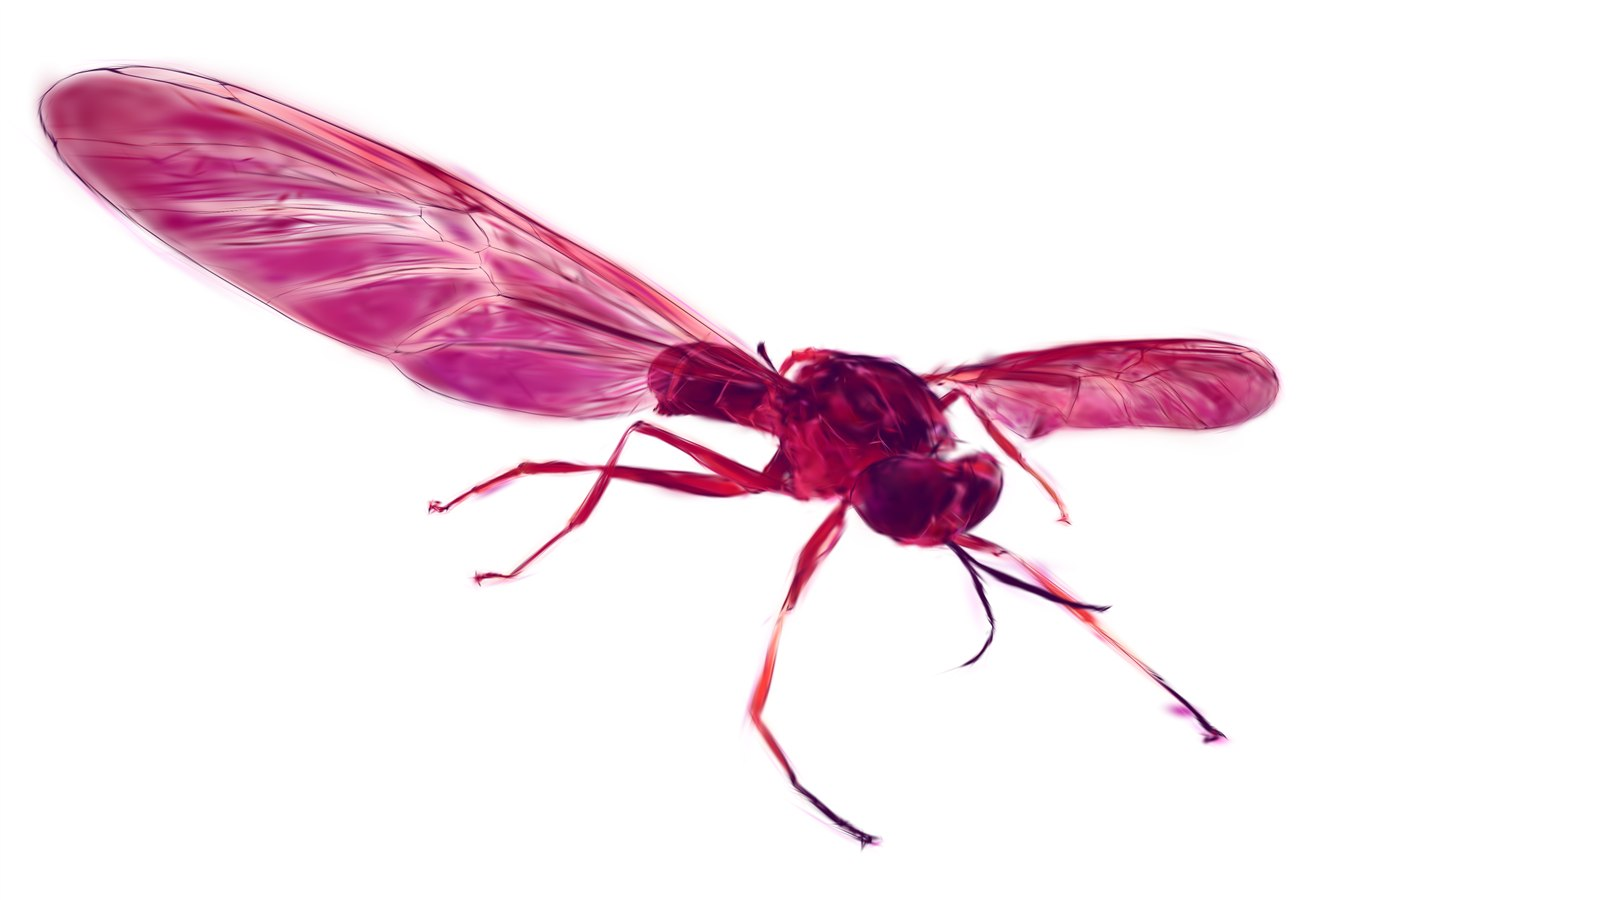
\includegraphics[width=0.24\linewidth]{imagens/artigo/im11.jpg}\hfill
  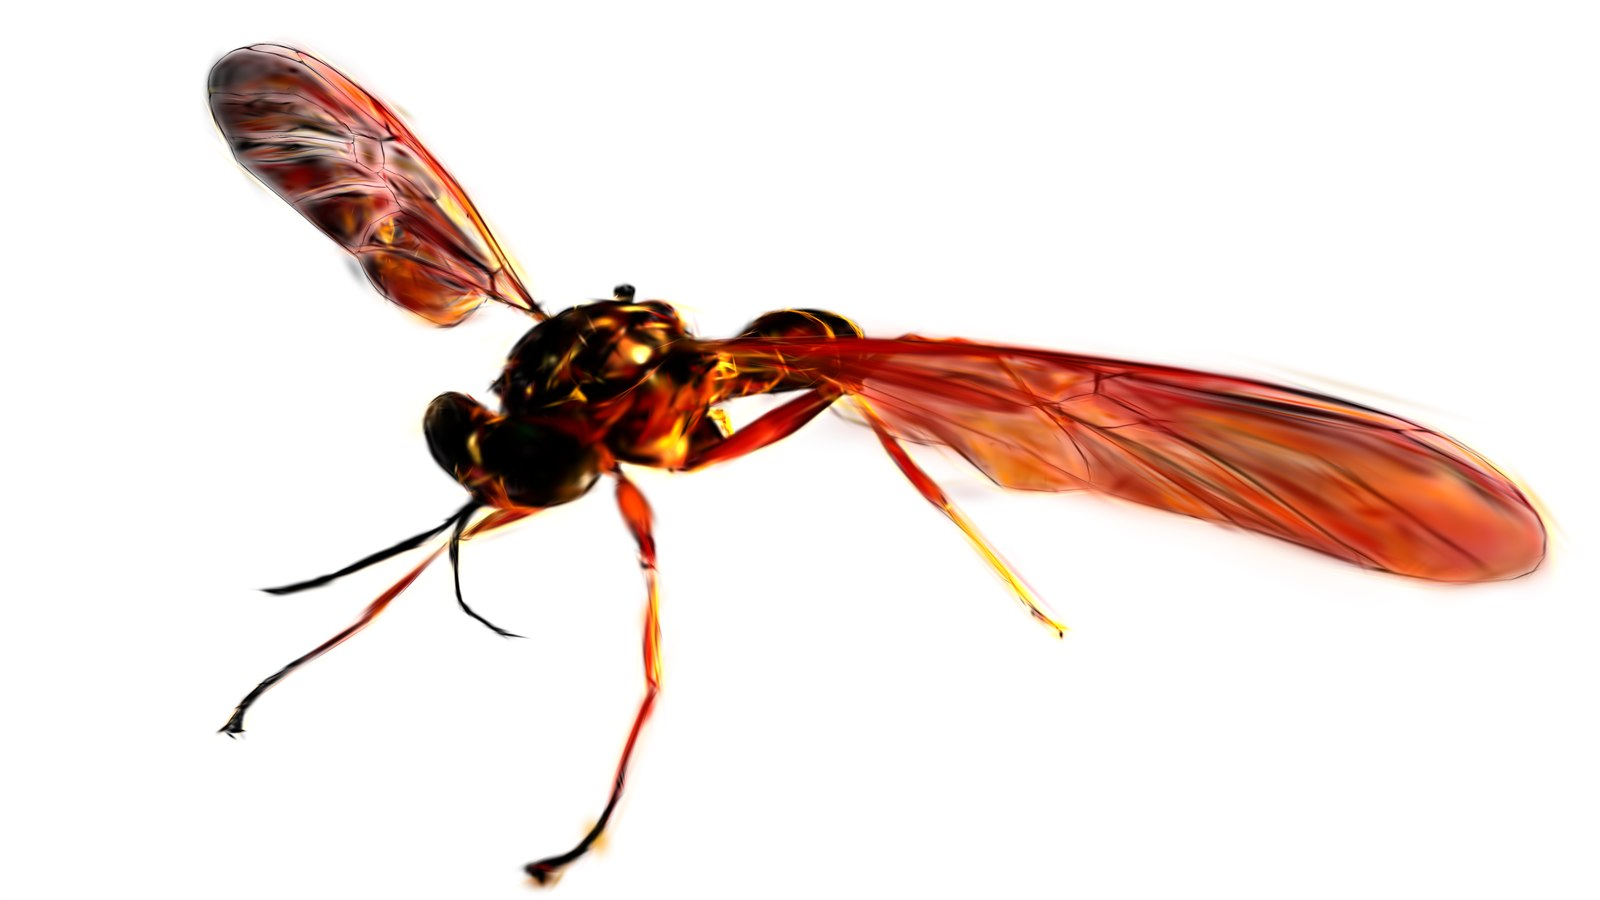
\includegraphics[width=0.24\linewidth]{imagens/artigo/im12.jpg}
  \caption{Saídas do \emph{pipeline} de RD Fotométrica aplicado aos modelos 3DGS da mariposa e da mosca.}
  \label{fig:fotometrica}
\end{figure}

\begin{figure}[htb]
  \centering
  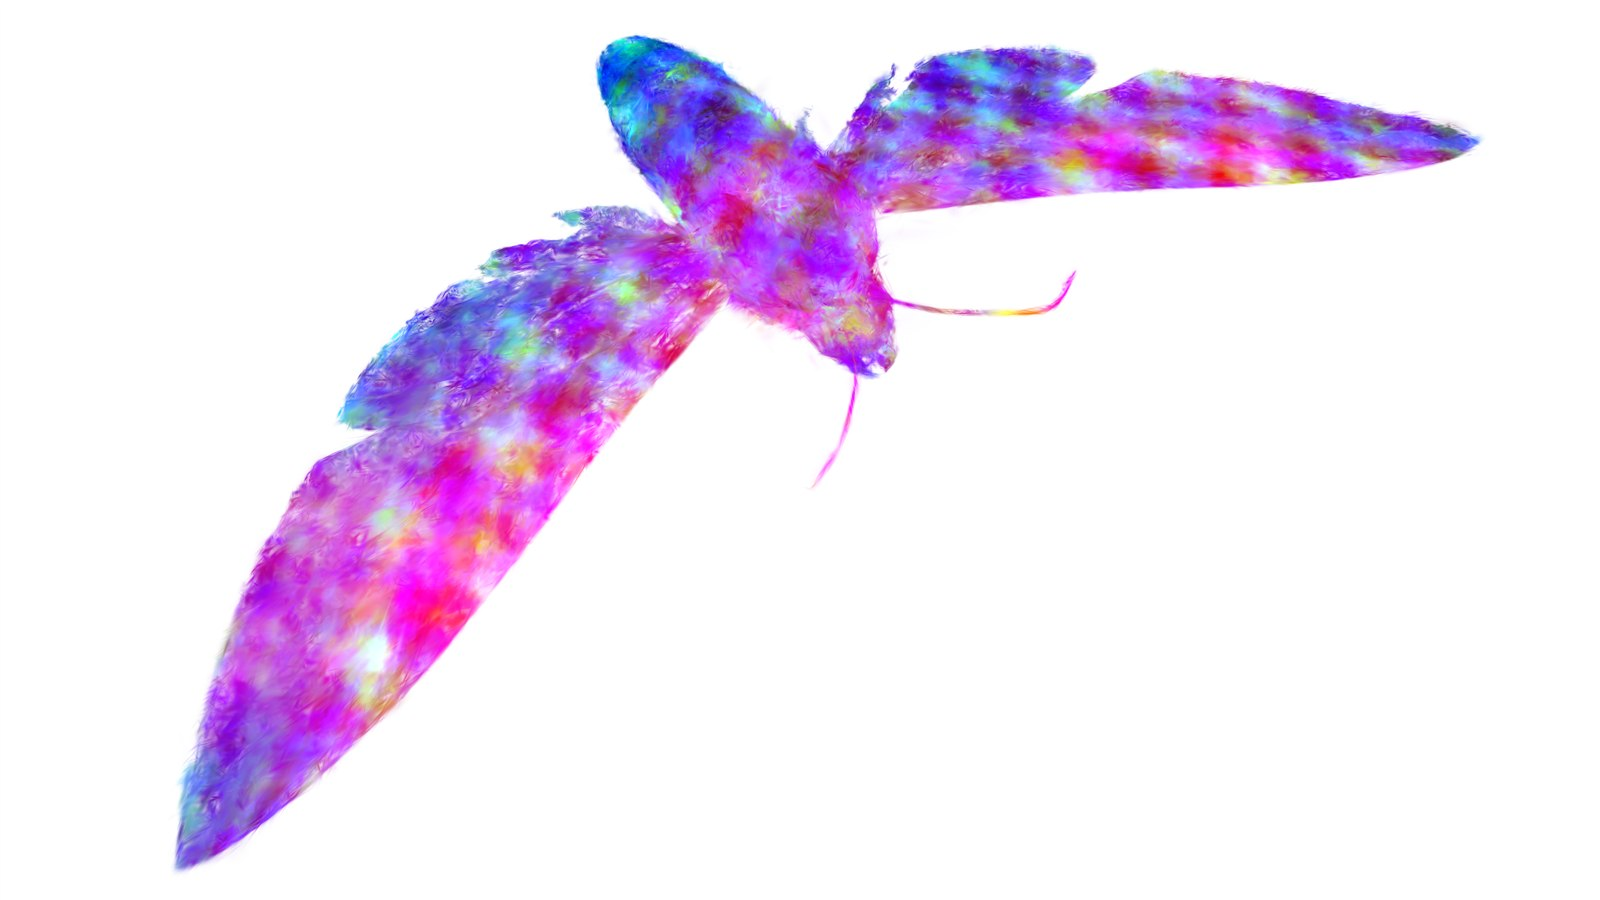
\includegraphics[width=0.24\linewidth]{imagens/artigo/im13.jpg}\hfill
  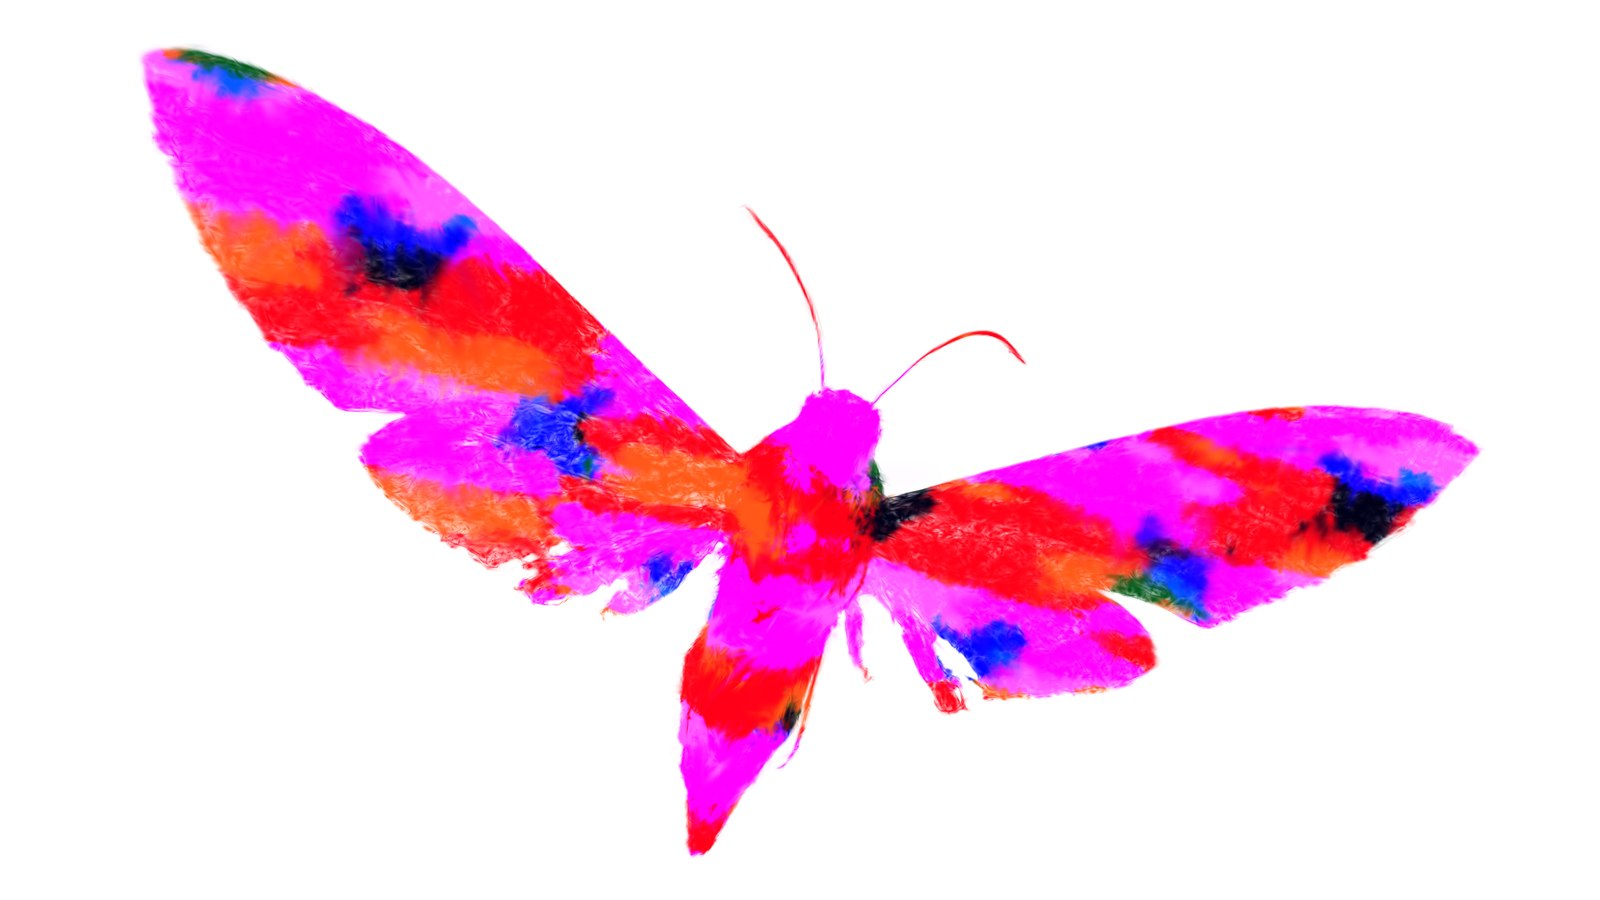
\includegraphics[width=0.24\linewidth]{imagens/artigo/im14.jpg}\hfill
  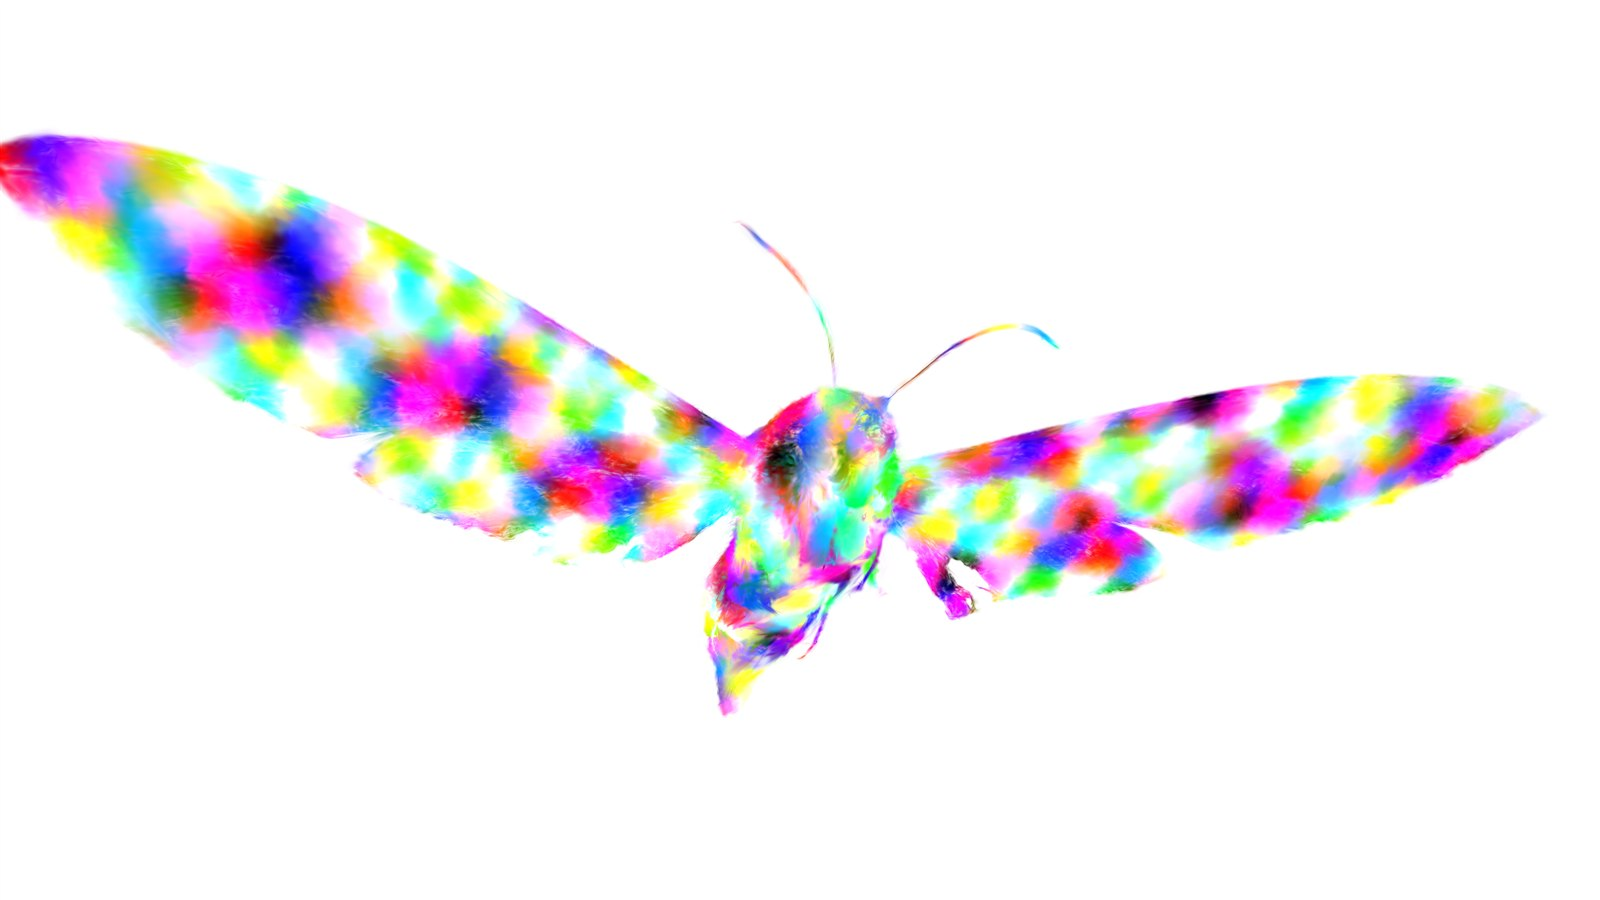
\includegraphics[width=0.24\linewidth]{imagens/artigo/im15.jpg}\hfill
  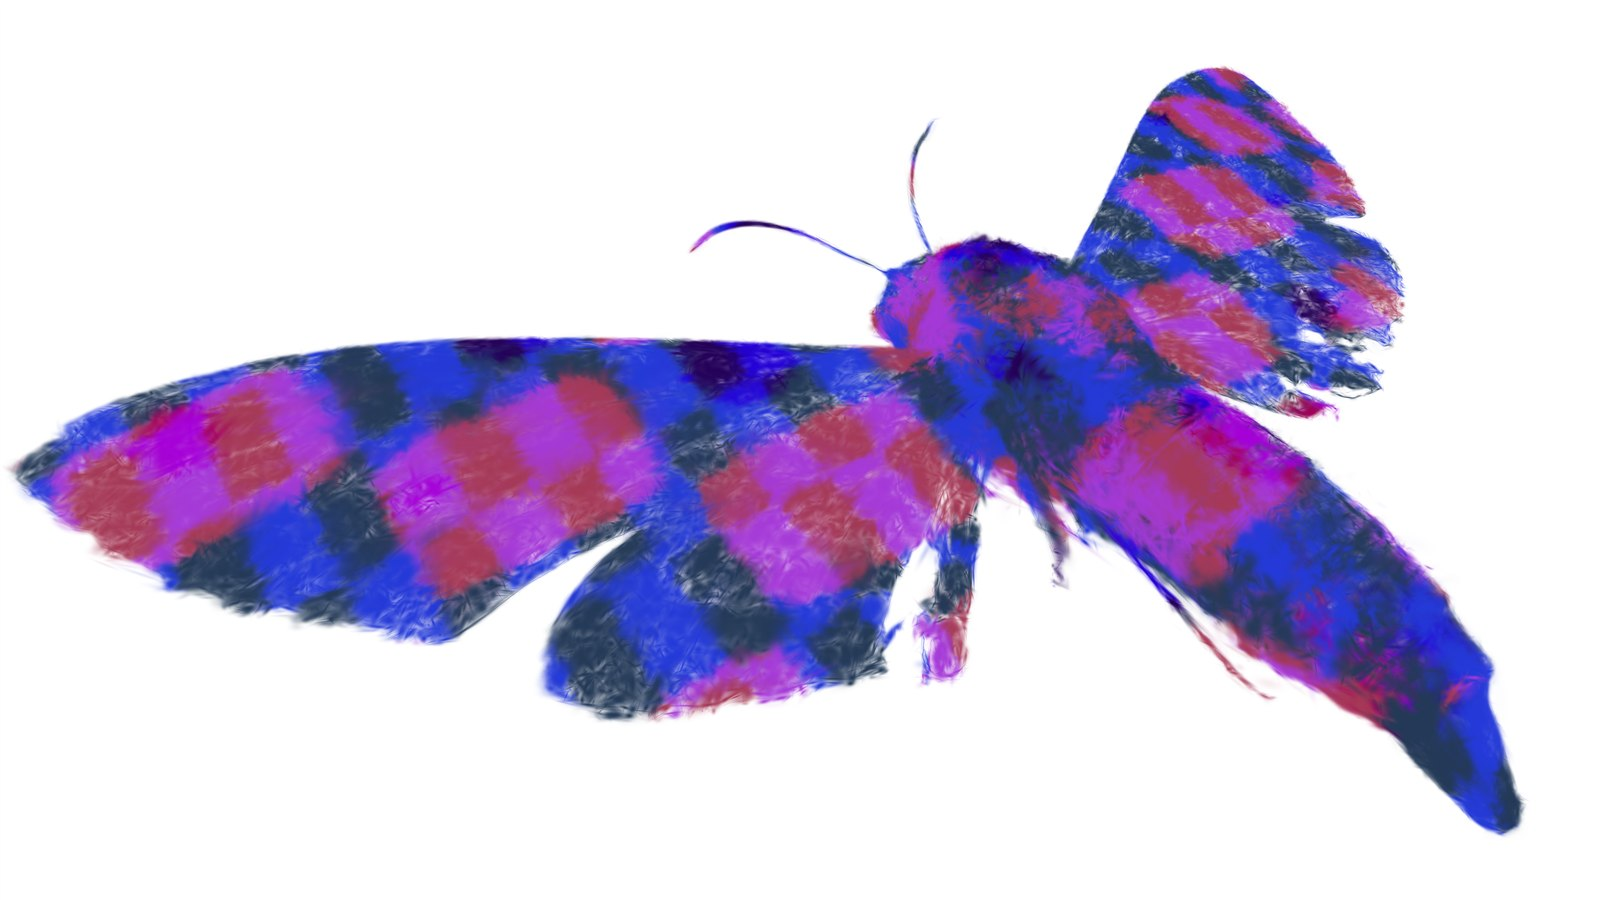
\includegraphics[width=0.24\linewidth]{imagens/artigo/im16.jpg}\\[2pt]
  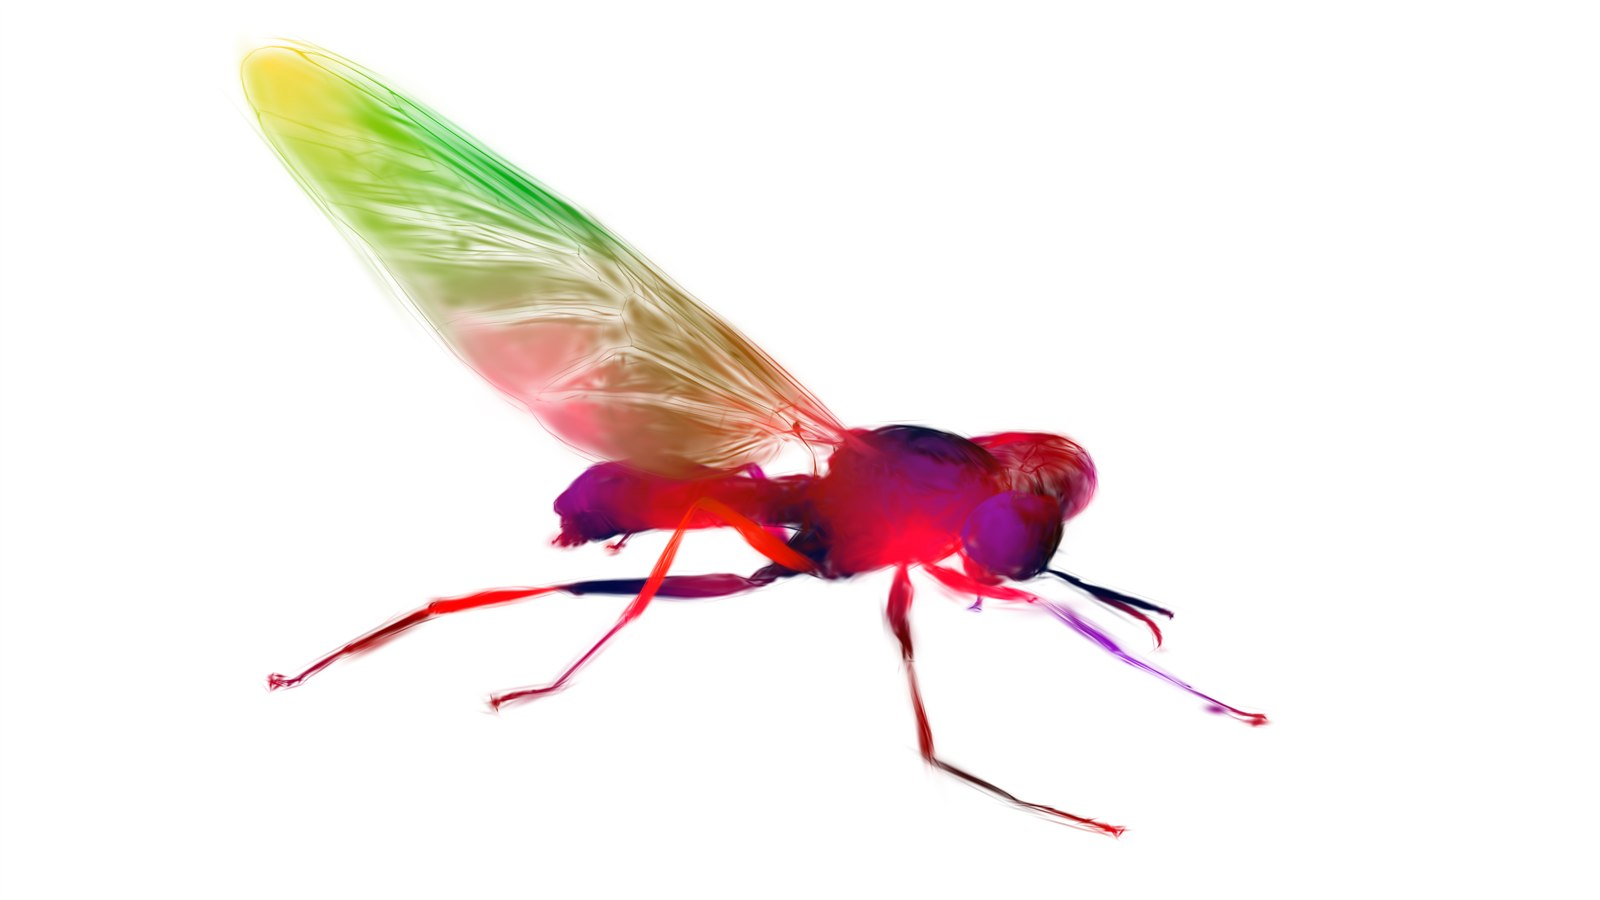
\includegraphics[width=0.24\linewidth]{imagens/artigo/im17.jpg}\hfill
  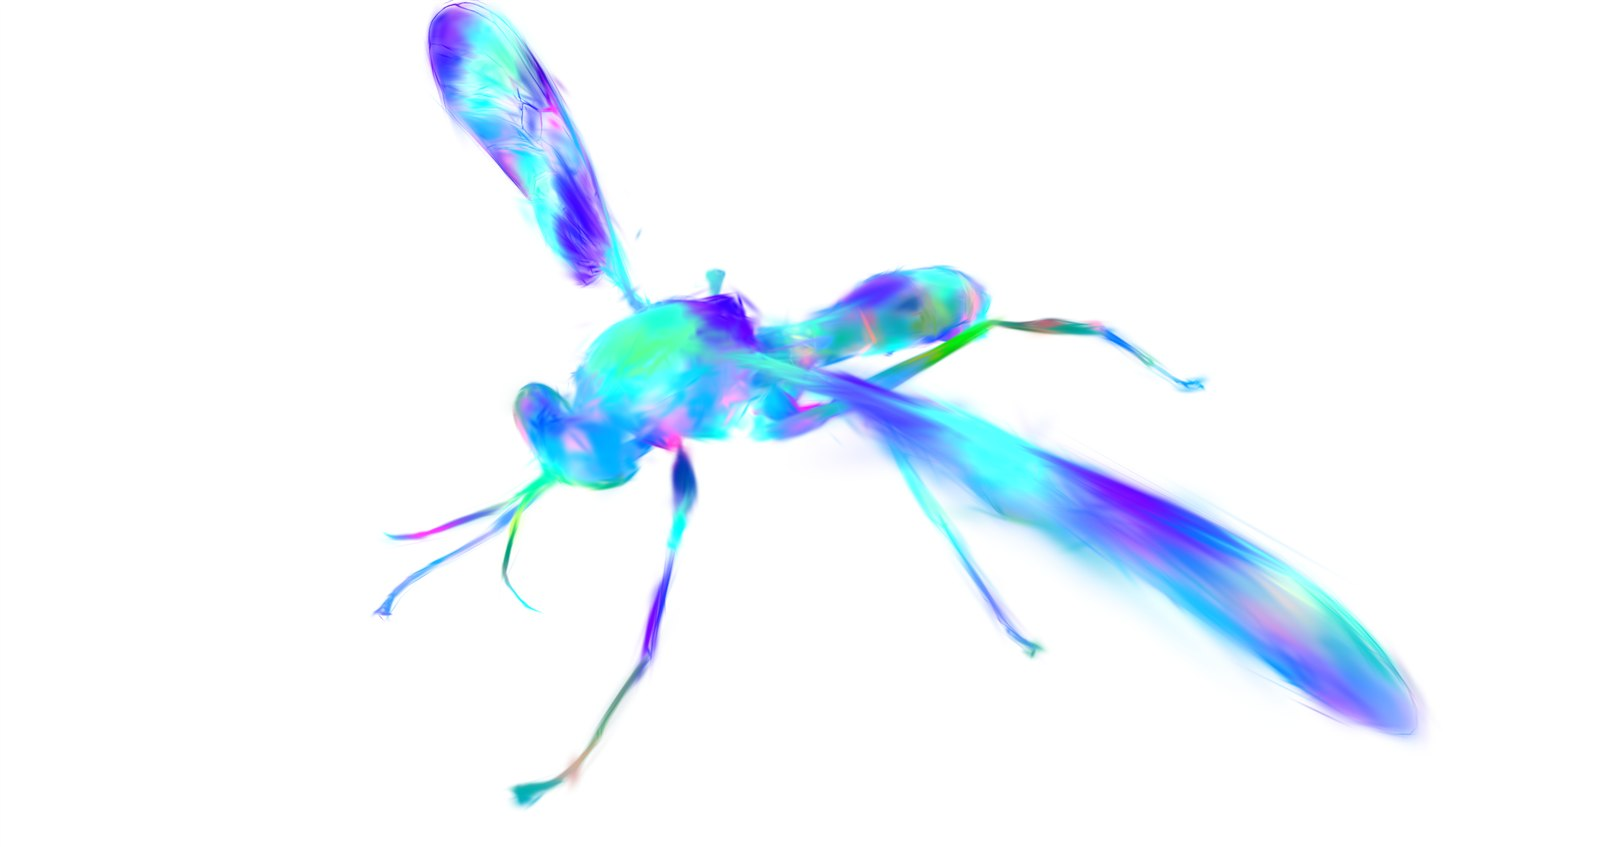
\includegraphics[width=0.24\linewidth]{imagens/artigo/im18.jpg}\hfill
  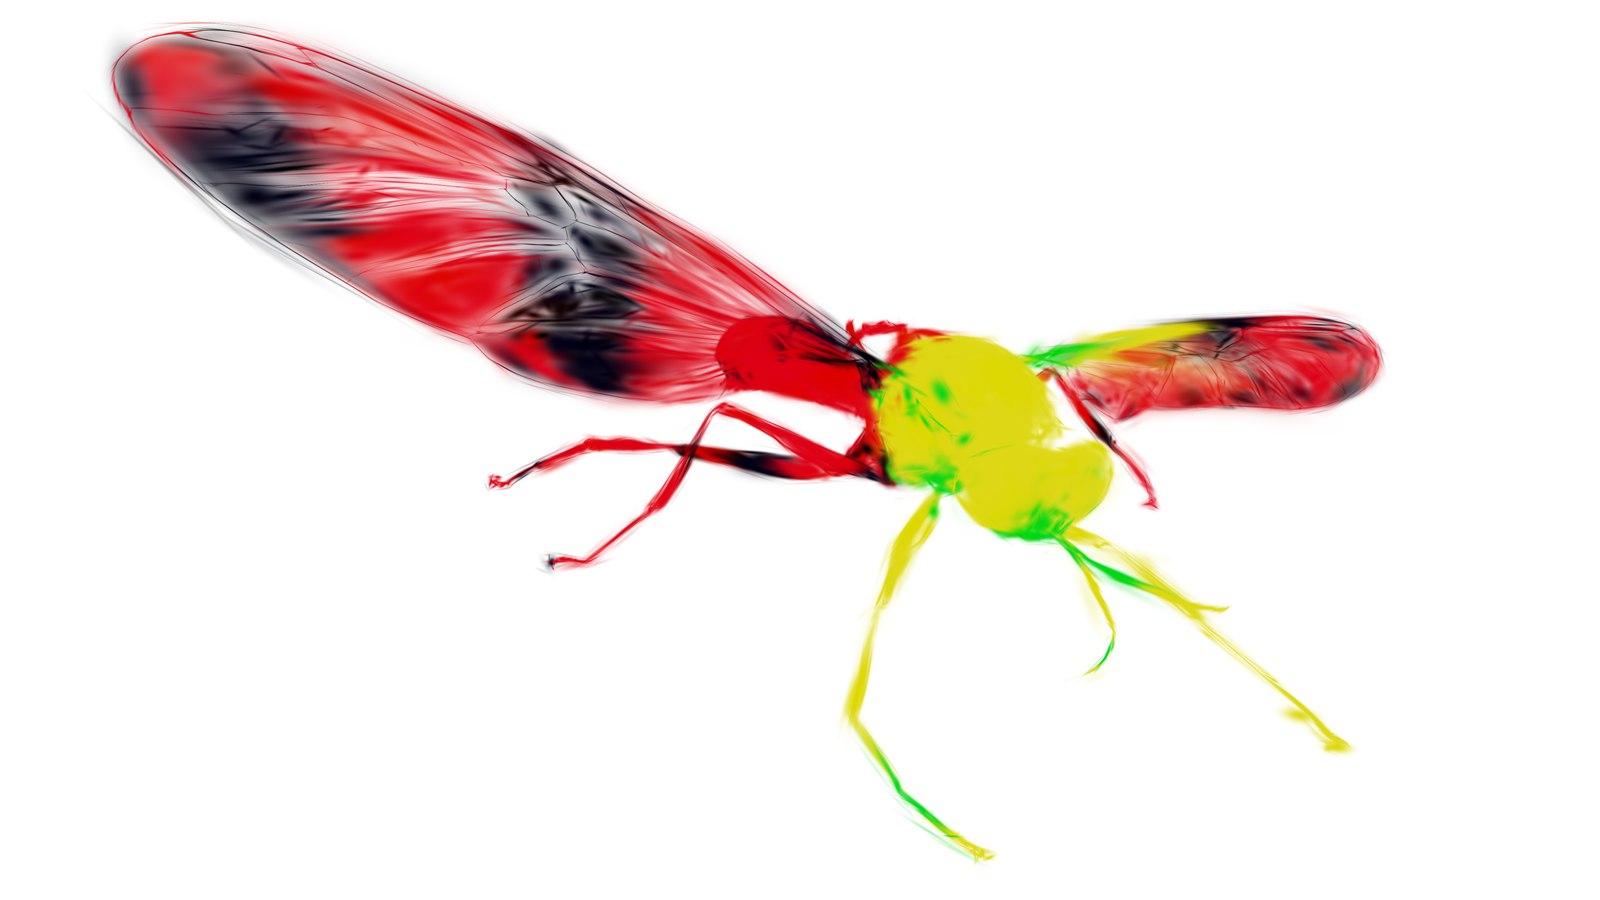
\includegraphics[width=0.24\linewidth]{imagens/artigo/im19.jpg}\hfill
  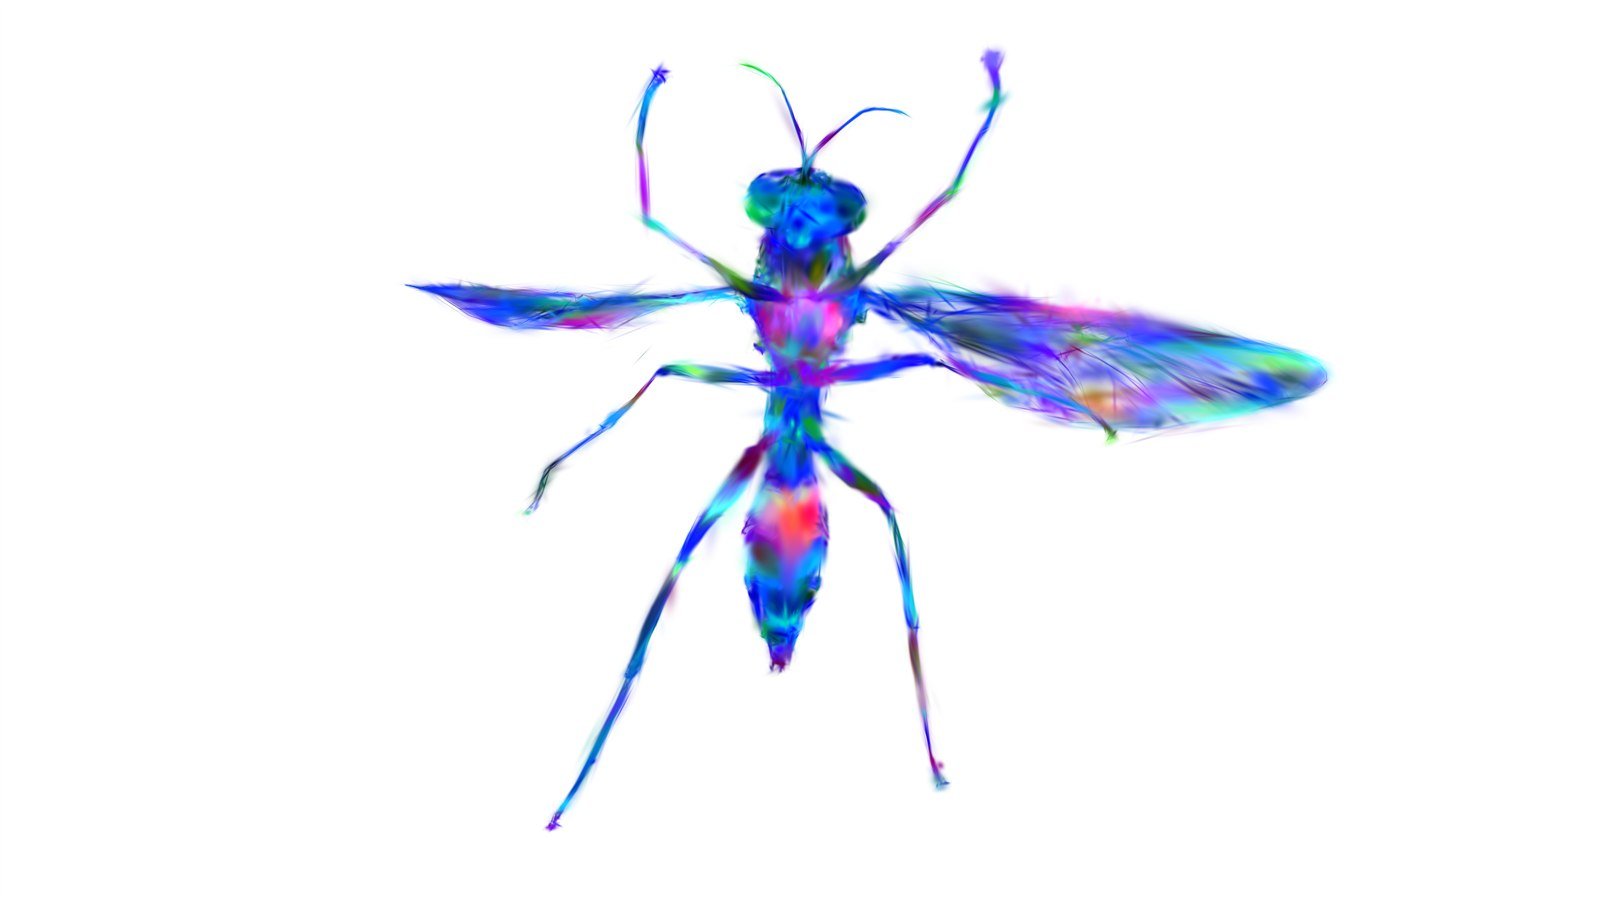
\includegraphics[width=0.24\linewidth]{imagens/artigo/im20.jpg}
  \caption{Saídas do \emph{pipeline} de RD Procedural. As texturas nativas são substituídas por mapeamentos de ruído espacial 3D, desacoplando a forma da aparência.}
  \label{fig:procedural}
\end{figure}


\subsection{Geração dos datasets (abcdataset)}

Os conjuntos gerados de tensores de parâmetros 3DGS randomizados são importados em uma aplicação Unity personalizada que executa um \emph{pipeline} dedicado de rasterização 3DGS \cite{pranckevicius2023unity}.

Esse ambiente funciona como um estúdio virtual automatizado, posicionando sequencialmente um sensor virtual em poses arbitrárias ao redor do \emph{asset}. O motor então compõe os espécimes biológicos 3D renderizados sobre um conjunto diversificado de texturas de fundo 2D amostradas estocasticamente e mapeadas em planos, terrenos e \emph{skyboxes}.

Durante a fase de rasterização, a \emph{bounding box} 2D é extraída projetando a \emph{bounding box} 3D do modelo no plano da imagem, o que fornece anotações 2D a custo zero para poses de câmera arbitrárias.

\subsection{Análise qualitativa inicial}

Para verificar se os \emph{pipelines} de perturbação expandem a variedade visual para além das capturas originais, realizou-se uma análise no espaço de características. Foram extraídos \emph{embeddings} profundos de alta dimensão utilizando uma arquitetura ResNet-50 pré-treinada \cite{he2016deep}, projetados em 2D com UMAP \cite{mcinnes2018umap}. O conjunto de avaliação foi estruturado em quatro categorias distintas de 100 imagens cada: (1) \emph{frames} de vídeo reais originais segmentados, com o fundo removido; (2) renderizações de controle, sem perturbação, do modelo 3DGS canônico; (3) renderizações randomizadas geradas pelos \emph{pipelines} de RD sobre fundo neutro; e (4) renderizações randomizadas compostas sobre fundos estocásticos. Para garantir uma fidelidade de base justa, as imagens canônicas de controle foram renderizadas a partir de poses de câmera alinhadas manualmente, próximas às trajetórias originais.

Para corroborar quantitativamente a análise visual do UMAP, calculou-se o \emph{Silhouette Score} \cite{rousseeuw1987silhouettes} para avaliar a separação entre os agrupamentos dos conjuntos reais e sintéticos no espaço de características de alta dimensão. Para um dado \emph{embedding} $i$, o \emph{silhouette score} $s(i)$ é definido como:
\begin{equation}
  s(i) = \frac{b(i) - a(i)}{\max\{a(i),\, b(i)\}},
\end{equation}
em que $a(i)$ representa a distância média intra-agrupamento entre o ponto $i$ e todos os demais pontos de sua própria categoria, e $b(i)$ denota a distância média a todos os pontos da categoria vizinha mais próxima. A métrica global $\bar{s}$ é a média aritmética de $s(i)$ sobre todos os $n$ pontos. Um valor próximo de 0 indica agrupamentos altamente sobrepostos ou adjacentes, enquanto um valor próximo de 1 indica maior separação espacial.

O valor de $\bar{s}$ foi avaliado para os espécimes de mariposa e de mosca em duas configurações distintas: (1) imagens reais originais segmentadas versus os modelos 3DGS canônicos sem perturbação; e (2) imagens reais originais segmentadas versus os modelos renderizados pelo \emph{pipeline} completo de RD.

\subsection{Avaliação Resnet50}

\subsection{Avaliação YOLO}


\subsection{Materiais e métodos}







 \section{Resultados e discussão}

Como ilustrado nas projeções UMAP tanto da mariposa (Fig.~\ref{fig:umap}a) quanto da mosca (Fig.~\ref{fig:umap}b), os \emph{embeddings} das renderizações 3DGS canônicas formam agrupamentos distintos e coesos. Embora visualmente semelhantes às capturas originais, esses agrupamentos apresentam um deslocamento espacial em relação às imagens reais. Essa separação é esperada e reflete a lacuna \emph{sim-to-real} típica de mídias sintetizadas, decorrente da suavização de texturas de alta frequência pelos Harmônicos Esféricos e de artefatos de rasterização subjacentes. Ainda assim, a densidade desses agrupamentos canônicos indica que os modelos de base permanecem morfologicamente consistentes.

A magnitude desse deslocamento inicial de domínio, entretanto, é desprezível quando comparada à dispersão introduzida pelos \emph{pipelines} de RD. Observa-se que os \emph{embeddings} dos modelos 3DGS randomizados expandem o domínio no espaço de características, superando as restrições de textura e iluminação das capturas originais. Essa ampla cobertura do espaço de características fornece os dados de treinamento variados necessários para favorecer a generalização \emph{sim-to-real}.

\begin{figure}[htb]
  \centering
  \begin{subfigure}{0.49\linewidth}
    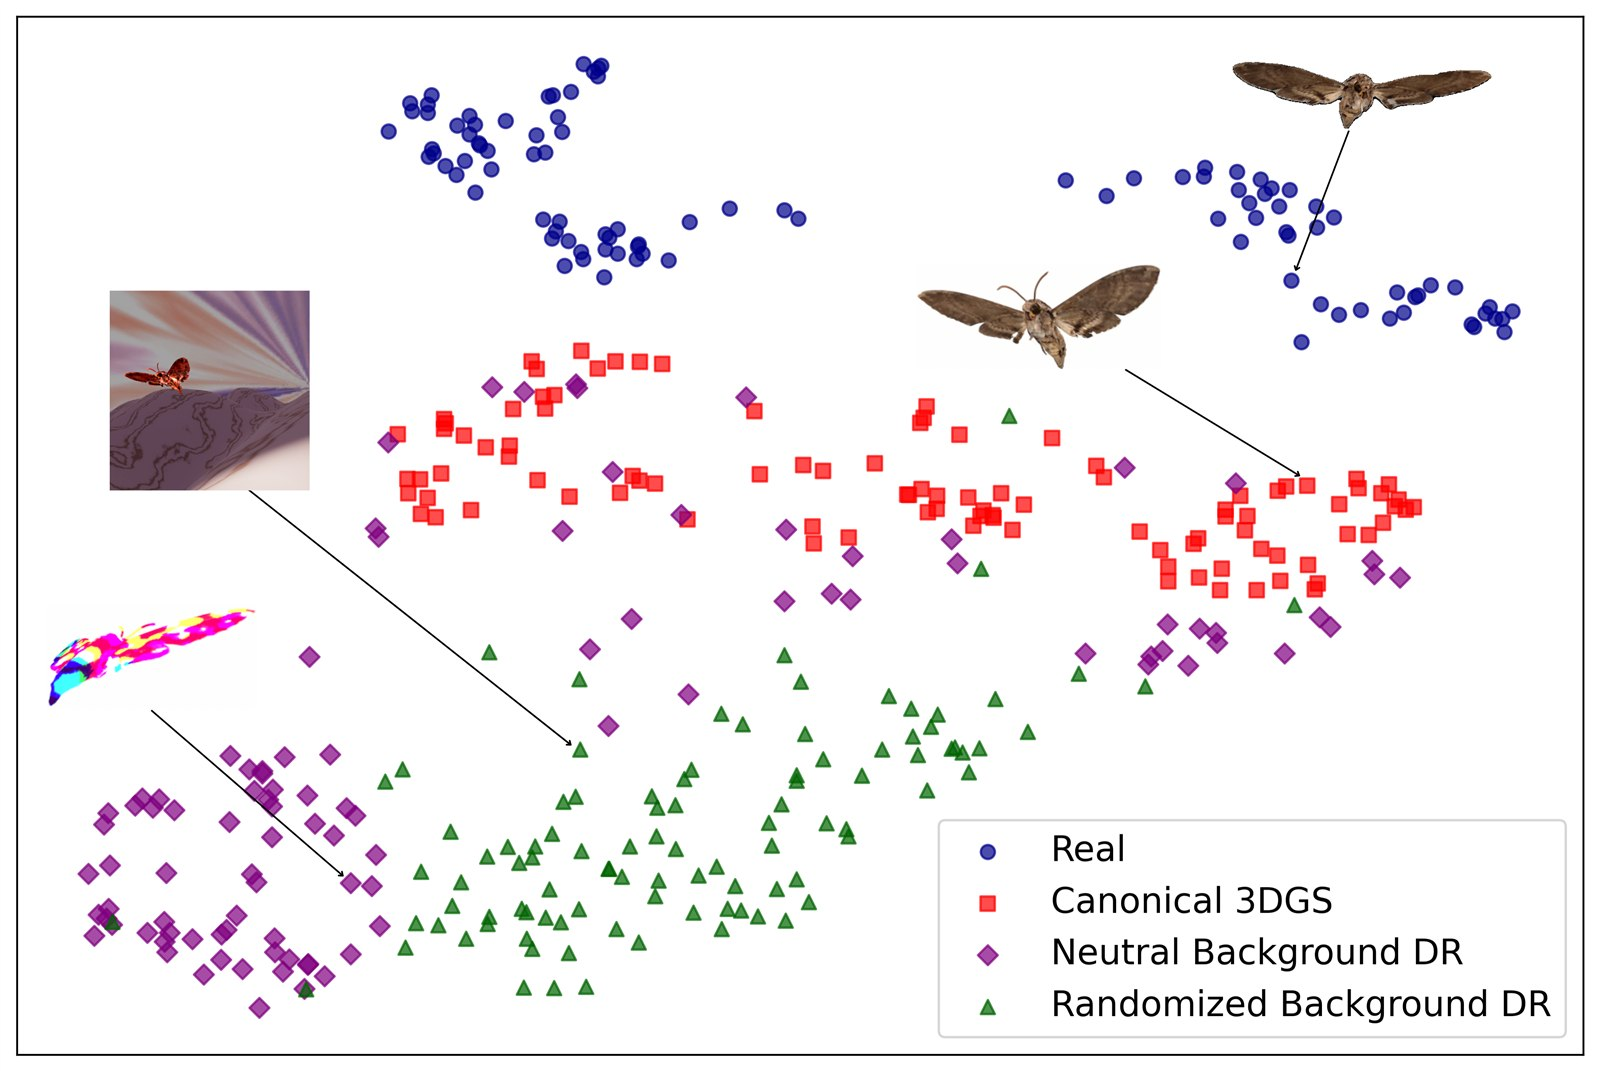
\includegraphics[width=\linewidth]{imagens/artigo/im21.jpg}
    \caption{Espécime de mariposa}
  \end{subfigure}\hfill
  \begin{subfigure}{0.49\linewidth}
    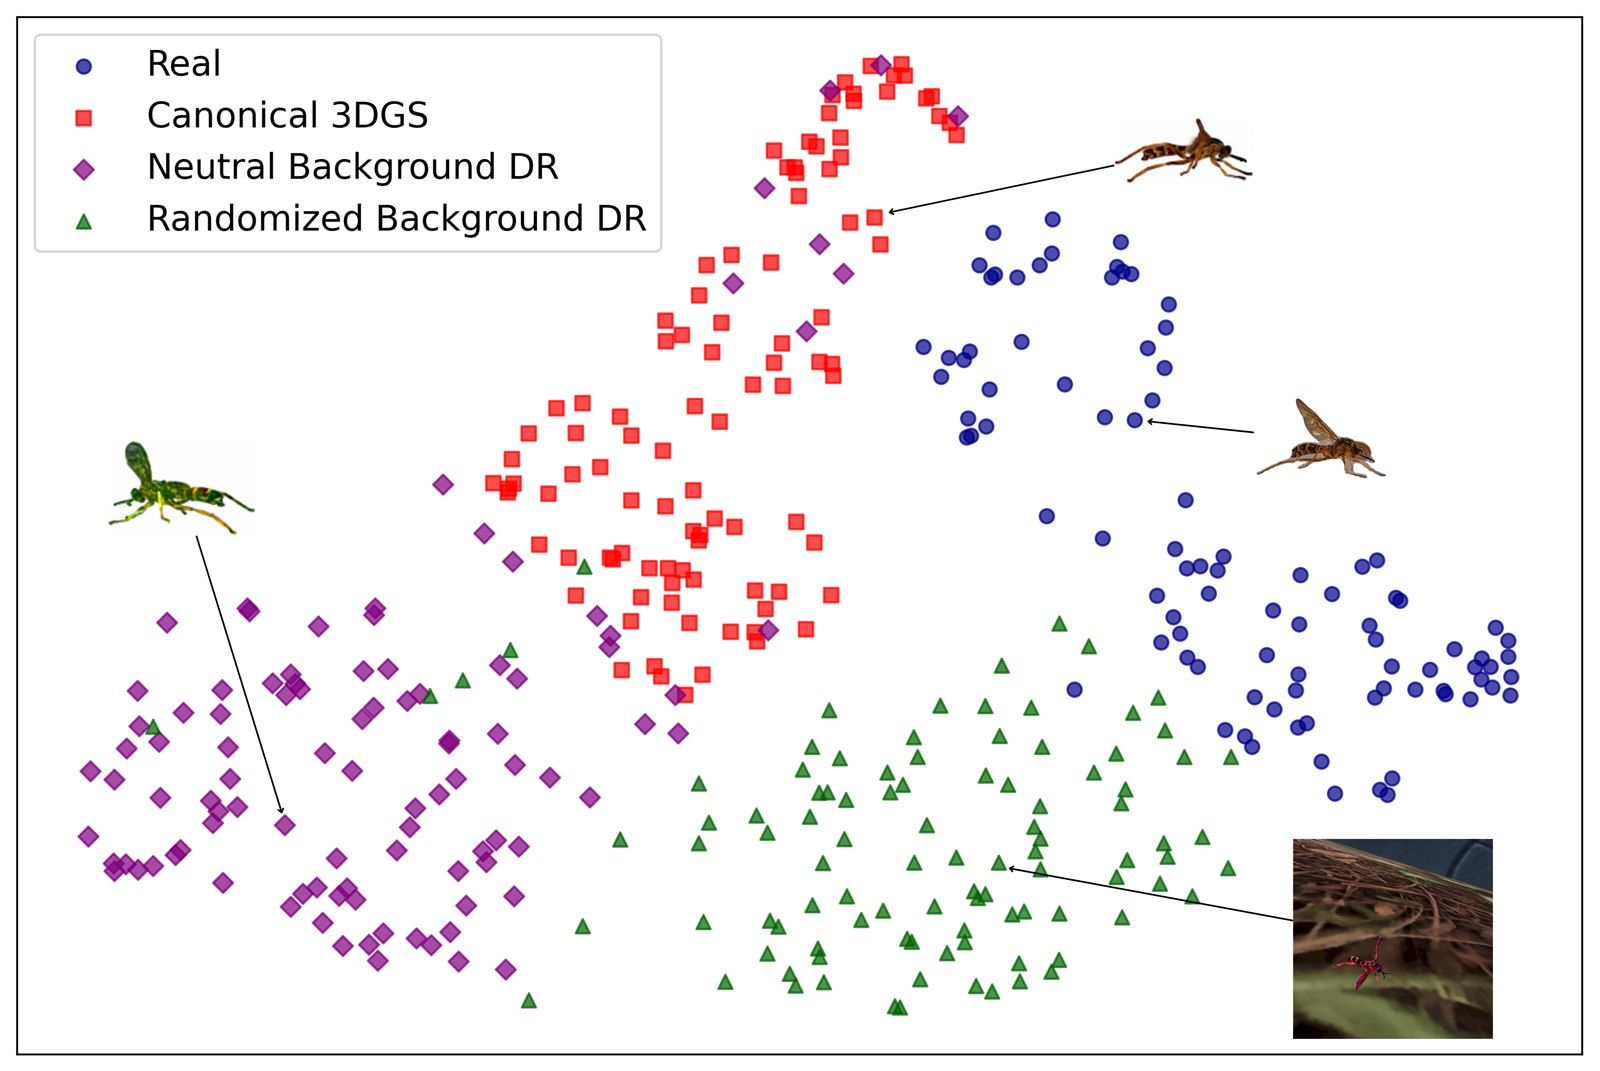
\includegraphics[width=\linewidth]{imagens/artigo/im22.jpg}
    \caption{Espécime de mosca}
  \end{subfigure}
  \caption{Projeções UMAP 2D dos \emph{embeddings} de uma ResNet-50 pré-treinada em quatro categorias: \emph{frames} de vídeo originais com o fundo removido (círculo azul-escuro), renderizações 3DGS canônicas sem perturbação (quadrado vermelho), renderizações de RD com fundo neutro (losango roxo) e renderizações de RD com fundo randomizado (triângulo verde).}
  \label{fig:umap}
\end{figure}

Na comparação com a base canônica, a avaliação resultou em um $\bar{s}$ baixo, de 0,1436 para a mariposa e 0,1532 para a mosca. Esses valores confirmam as pequenas lacunas de renderização observadas nas projeções UMAP, reforçando que as reconstruções 3DGS sem perturbação atuam como representações confiáveis e morfologicamente próximas dos espécimes reais. Em contraste, ao avaliar a configuração completa de RD, $\bar{s}$ aumentou para 0,2235 para a mariposa e 0,1847 para a mosca. Esse aumento mensurável confirma que o \emph{pipeline} de RD expande a variância no espaço de características. A magnitude conservadora desse aumento indica uma expansão controlada: embora seja introduzida diversidade visual suficiente para superar vieses texturais, a identidade morfológica subjacente dos espécimes é preservada, garantindo que os dados sintéticos permaneçam semanticamente ancorados ao domínio real.

\subsection{Limitações}

Embora o \emph{framework} de RD proposto expanda a variância visual das representações 3DGS, ele está sujeito a restrições técnicas e físicas.

Primeiro, há uma limitação óptica decorrente do uso de macrofotografia. Capturar pequenos espécimes biológicos com configurações multivista casuais em dispositivos móveis convencionais resulta em pouca profundidade de campo e em desfoque ao longo dos \emph{frames} de vídeo. Mitigar esse problema tradicionalmente exige protocolos de empilhamento de foco (\emph{focus stacking}), que demandam equipamento dedicado, penalizam a vazão de aquisição e são proibitivos para capturas dinâmicas \cite{berger2025rapid}. As reconstruções 3DGS canônicas herdam esses artefatos de desfoque, o que pode degradar a fidelidade de base dos campos de radiância otimizados.

Segundo, a geometria permanece rígida. Embora seja possível randomizar continuamente a aparência para superar vieses de textura, ainda não é possível animar poses anatômicas articuladas, como a variação dos ângulos diedros das asas ou das articulações das pernas dos insetos.

Terceiro, o 3DGS padrão apresenta uma representação entrelaçada de materiais e iluminação. Como o campo de radiância explícito incorpora a iluminação ambiental original, os espécimes importados não respondem dinamicamente aos sistemas de iluminação física nativos do motor de rasterização (por exemplo, às luzes direcionais ou às sombras em tempo real do Unity). Além disso, no \emph{pipeline} de perturbação fotométrica, manipular e rotacionar corretamente a iluminação é matematicamente simples para os SH de ordem zero e um; no entanto, rotacionar com precisão os coeficientes de ordem superior, preservando especularidades complexas e dependentes do ponto de vista sob reorientações espaciais arbitrárias, continua sendo computacionalmente desafiador. Consequentemente, o \emph{pipeline} recorre ao escalonamento de intensidade para essas ordens superiores.

Por fim, do ponto de vista da arquitetura de software, a implementação atual opera como um \emph{pipeline} desacoplado de dois estágios: os tensores perturbados são pré-calculados em Python e exportados como arquivos \texttt{.ply} antes de serem carregados no Unity. Uma arquitetura unificada, na qual a manipulação de tensores e a rasterização ocorram simultaneamente na memória da GPU, seria necessária para eliminar gargalos de E/S em disco e maximizar a vazão de geração dos \emph{datasets}.




 
\newpage


\bibliography{bibliografia.bib}



\end{document}
